% Fixed-population analysis. Numerical inputs: generated/ch3_transport_report.json.
\chapter{Horizontal transport and displacement scaling}
\label{ch:fixed-transport}
% Generated by scripts/tesi/ch03_fixed_transport/write_ch3_text.py
% Chapter prose is hand-written; only these values are generated.
\newcommand{\ChThreeClosedAltShiftMax}{0.051}
\newcommand{\ChThreeClosedAltShiftMin}{0.021}
\newcommand{\ChThreeCohortBiasMaxPct}{2.0}
\newcommand{\ChThreeCohortBiasMinPct}{1.8}
\newcommand{\ChThreeCohortShiftMax}{0.0177}
\newcommand{\ChThreeCohortShiftMin}{0.0164}
\newcommand{\ChThreeEligibleClosed}{87,807}
\newcommand{\ChThreeEligibleClosedPct}{56.6}
\newcommand{\ChThreeEligibleOpen}{67,003}
\newcommand{\ChThreeEligibleOpenPct}{43.2}
\newcommand{\ChThreeEligibleUnknown}{275}
\newcommand{\ChThreeGeneralFitLagMax}{30000}
\newcommand{\ChThreeGeneralFitLagMin}{10}
\newcommand{\ChThreeGeneralLastFitLag}{28440}
\newcommand{\ChThreeHangClosedFracMain}{76.5}
\newcommand{\ChThreeHangClosedFracStart}{64.0}
\newcommand{\ChThreeHangCohortOverlapPct}{99.7}
\newcommand{\ChThreeHangGeneralGroups}{7}
\newcommand{\ChThreeHangGeneralHurst}{0.841 [0.816, 0.855]}
\newcommand{\ChThreeHangGeneralReplicates}{998}
\newcommand{\ChThreeHangGeneralRms}{0.075}
\newcommand{\ChThreeHangGeneralRmsRatio}{1.19}
\newcommand{\ChThreeHangKurtEEnd}{4.03}
\newcommand{\ChThreeHangKurtEStart}{-0.60}
\newcommand{\ChThreeHangKurtNEnd}{2.24}
\newcommand{\ChThreeHangKurtNStart}{-0.72}
\newcommand{\ChThreeHangLastSupportLag}{43200}
\newcommand{\ChThreeHangLocalMinH}{0.57}
\newcommand{\ChThreeHangLocalMinLag}{320}
\newcommand{\ChThreeHangMomentContrast}{-0.0085 [-0.0112, -0.0057]}
\newcommand{\ChThreeHangMomentRmsMax}{0.126}
\newcommand{\ChThreeHangMomentRmsMin}{0.011}
\newcommand{\ChThreeHangPriorInterp}{9,648}
\newcommand{\ChThreeHangQuantRatioEnd}{0.233}
\newcommand{\ChThreeHangQuantRatioMax}{0.385}
\newcommand{\ChThreeHangQuantRatioMaxLag}{1970}
\newcommand{\ChThreeHangQuantRatioMin}{0.192}
\newcommand{\ChThreeHangQuantRatioMinLag}{90}
\newcommand{\ChThreeHangQuantRatioStart}{0.472}
\newcommand{\ChThreeHangQuantRmsMax}{0.101}
\newcommand{\ChThreeHangQuantRmsMin}{0.037}
\newcommand{\ChThreeMainClosed}{28,234}
\newcommand{\ChThreeMainClosedPct}{61.0}
\newcommand{\ChThreeMainOpen}{17,961}
\newcommand{\ChThreeMainOpenPct}{38.8}
\newcommand{\ChThreeMainUnknown}{78}
\newcommand{\ChThreeOpenAltShiftMax}{0.064}
\newcommand{\ChThreeOpenAltShiftMin}{0.051}
\newcommand{\ChThreeParaClosedFracMain}{61.0}
\newcommand{\ChThreeParaClosedFracStart}{56.6}
\newcommand{\ChThreeParaCohortOverlapPct}{99.6}
\newcommand{\ChThreeParaGeneralHurst}{0.869 [0.864, 0.874]}
\newcommand{\ChThreeParaGeneralRms}{0.038}
\newcommand{\ChThreeParaGeneralRmsRatio}{1.09}
\newcommand{\ChThreeParaKurtEEnd}{2.77}
\newcommand{\ChThreeParaKurtEStart}{-0.68}
\newcommand{\ChThreeParaKurtNEnd}{0.94}
\newcommand{\ChThreeParaKurtNStart}{-0.97}
\newcommand{\ChThreeParaLastSupportLag}{32690}
\newcommand{\ChThreeParaLocalMinH}{0.66}
\newcommand{\ChThreeParaLocalMinLag}{110}
\newcommand{\ChThreeParaMomentContrast}{0.0095 [0.0086, 0.0105]}
\newcommand{\ChThreeParaMomentRmsMax}{0.079}
\newcommand{\ChThreeParaMomentRmsMin}{0.010}
\newcommand{\ChThreeParaPriorInterp}{355,170}
\newcommand{\ChThreeParaQuantRatioEnd}{0.205}
\newcommand{\ChThreeParaQuantRatioMax}{0.398}
\newcommand{\ChThreeParaQuantRatioMaxLag}{1970}
\newcommand{\ChThreeParaQuantRatioMin}{0.244}
\newcommand{\ChThreeParaQuantRatioMinLag}{100}
\newcommand{\ChThreeParaQuantRatioStart}{0.510}
\newcommand{\ChThreeParaQuantRmsMax}{0.084}
\newcommand{\ChThreeParaQuantRmsMin}{0.023}
\newcommand{\ChThreeTaskContrastMax}{0.129}
\newcommand{\ChThreeTaskContrastMin}{0.023}
\newcommand{\ChThreeTaskGapHigh}{0.023 [0.021, 0.024]}
\newcommand{\ChThreeTaskGapHills}{0.129 [0.125, 0.132]}
\newcommand{\ChThreeTaskGapLow}{0.048 [0.046, 0.049]}
\newcommand{\ChThreeTaskGapPlains}{0.128 [0.120, 0.138]}

% Generated values only; prose is maintained in the chapter.
\newcommand{\ChThreeHangGridGroups}{267}
\newcommand{\ChThreeHangGridHFactor}{2.00--2.05}
\newcommand{\ChThreeHangGridHThreeMonths}{1.40}
\newcommand{\ChThreeHangGridMaxPct}{13.4}
\newcommand{\ChThreeHangGridMedian}{2}
\newcommand{\ChThreeHangGridMsdShiftRange}{0.98--1.87}
\newcommand{\ChThreeHangGridOldSingletonPct}{81.3}
\newcommand{\ChThreeHangGridSingletonFlightPct}{5.0}
\newcommand{\ChThreeHangGridSingletonPct}{43.4}
\newcommand{\ChThreeParaGridGroups}{1901}
\newcommand{\ChThreeParaGridHFactor}{3.97--4.05}
\newcommand{\ChThreeParaGridHThreeMonths}{1.49}
\newcommand{\ChThreeParaGridMaxPct}{4.4}
\newcommand{\ChThreeParaGridMedian}{3}
\newcommand{\ChThreeParaGridMsdShiftRange}{0.98--1.04}
\newcommand{\ChThreeParaGridOldSingletonPct}{71.1}
\newcommand{\ChThreeParaGridSingletonFlightPct}{1.4}
\newcommand{\ChThreeParaGridSingletonPct}{33.5}

% Generated by check_origin_dependence.py
\newcommand{\ChThreeHangOriginDeltaH}{-0.0168}
\newcommand{\ChThreeHangOriginDeltaHHigh}{-0.0150}
\newcommand{\ChThreeHangOriginDeltaHLow}{-0.0186}
\newcommand{\ChThreeHangOriginPeak}{1.337}
\newcommand{\ChThreeHangOriginPeakInterval}{1.310--1.364}
\newcommand{\ChThreeHangOriginPeakLag}{390}
\newcommand{\ChThreeHangOriginPeakLever}{11489}
\newcommand{\ChThreeHangOriginResolved}{32}
\newcommand{\ChThreeParaOriginDeltaH}{-0.0104}
\newcommand{\ChThreeParaOriginDeltaHHigh}{-0.0098}
\newcommand{\ChThreeParaOriginDeltaHLow}{-0.0110}
\newcommand{\ChThreeParaOriginPeak}{1.388}
\newcommand{\ChThreeParaOriginPeakInterval}{1.378--1.398}
\newcommand{\ChThreeParaOriginPeakLag}{390}
\newcommand{\ChThreeParaOriginPeakLever}{12100}
\newcommand{\ChThreeParaOriginResolved}{33}

% Generated conditional transport measurements.
\newcommand{\CondAllH}{$0.882\;[0.881,\,0.883]$}
\newcommand{\CondAllN}{46273}
\newcommand{\CondOpenH}{$0.910\;[0.909,\,0.911]$}
\newcommand{\CondOpenN}{17961}
\newcommand{\CondClosedH}{$0.856\;[0.855,\,0.856]$}
\newcommand{\CondClosedN}{28234}
\newcommand{\CondAltZeroH}{$0.950\;[0.948,\,0.951]$}
\newcommand{\CondAltZeroN}{1844}
\newcommand{\CondOpenZeroH}{$0.953\;[0.952,\,0.955]$}
\newcommand{\CondOpenZeroN}{1679}
\newcommand{\CondClosedZeroH}{$0.825\;[0.816,\,0.834]$}
\newcommand{\CondClosedZeroN}{165}
\newcommand{\CondAltOneH}{$0.929\;[0.926,\,0.931]$}
\newcommand{\CondAltOneN}{2908}
\newcommand{\CondOpenOneH}{$0.944\;[0.943,\,0.946]$}
\newcommand{\CondOpenOneN}{2068}
\newcommand{\CondClosedOneH}{$0.816\;[0.812,\,0.819]$}
\newcommand{\CondClosedOneN}{839}
\newcommand{\CondAltTwoH}{$0.866\;[0.865,\,0.867]$}
\newcommand{\CondAltTwoN}{22097}
\newcommand{\CondOpenTwoH}{$0.893\;[0.892,\,0.895]$}
\newcommand{\CondOpenTwoN}{7412}
\newcommand{\CondClosedTwoH}{$0.846\;[0.845,\,0.847]$}
\newcommand{\CondClosedTwoN}{14649}
\newcommand{\CondAltThreeH}{$0.875\;[0.874,\,0.876]$}
\newcommand{\CondAltThreeN}{19424}
\newcommand{\CondOpenThreeH}{$0.889\;[0.888,\,0.890]$}
\newcommand{\CondOpenThreeN}{6802}
\newcommand{\CondClosedThreeH}{$0.866\;[0.865,\,0.867]$}
\newcommand{\CondClosedThreeN}{12581}
\newcommand{\CondMountainsH}{$0.871\;[0.870,\,0.871]$}
\newcommand{\CondMountainsN}{41521}
\newcommand{\CondLowlandsH}{$0.938\;[0.936,\,0.939]$}
\newcommand{\CondLowlandsN}{4752}
\newcommand{\CondBeginnersH}{$0.870\;[0.869,\,0.871]$}
\newcommand{\CondBeginnersN}{27609}
\newcommand{\CondBeginnersMountainsH}{$0.862\;[0.862,\,0.863]$}
\newcommand{\CondBeginnersMountainsN}{25691}
\newcommand{\CondBeginnersLowlandsH}{$0.928\;[0.926,\,0.930]$}
\newcommand{\CondBeginnersLowlandsN}{1918}
\newcommand{\CondBeginnersAltZeroH}{$0.940\;[0.937,\,0.942]$}
\newcommand{\CondBeginnersAltZeroN}{703}
\newcommand{\CondBeginnersAltOneH}{$0.920\;[0.917,\,0.923]$}
\newcommand{\CondBeginnersAltOneN}{1215}
\newcommand{\CondBeginnersAltTwoH}{$0.857\;[0.856,\,0.858]$}
\newcommand{\CondBeginnersAltTwoN}{13757}
\newcommand{\CondBeginnersAltThreeH}{$0.868\;[0.867,\,0.869]$}
\newcommand{\CondBeginnersAltThreeN}{11934}
\newcommand{\CondExpertsH}{$0.895\;[0.893,\,0.896]$}
\newcommand{\CondExpertsN}{16497}
\newcommand{\CondExpertsMountainsH}{$0.881\;[0.880,\,0.882]$}
\newcommand{\CondExpertsMountainsN}{14038}
\newcommand{\CondExpertsLowlandsH}{$0.942\;[0.940,\,0.943]$}
\newcommand{\CondExpertsLowlandsN}{2459}
\newcommand{\CondExpertsAltZeroH}{$0.953\;[0.951,\,0.954]$}
\newcommand{\CondExpertsAltZeroN}{955}
\newcommand{\CondExpertsAltOneH}{$0.933\;[0.930,\,0.935]$}
\newcommand{\CondExpertsAltOneN}{1504}
\newcommand{\CondExpertsAltTwoH}{$0.878\;[0.876,\,0.879]$}
\newcommand{\CondExpertsAltTwoN}{7390}
\newcommand{\CondExpertsAltThreeH}{$0.884\;[0.883,\,0.885]$}
\newcommand{\CondExpertsAltThreeN}{6648}
\newcommand{\CondAlpsH}{$0.870\;[0.870,\,0.871]$}
\newcommand{\CondAlpsN}{32790}
\newcommand{\CondAlpsExcluded}{385}
\newcommand{\CondPyreneesH}{$0.833\;[0.829,\,0.837]$}
\newcommand{\CondPyreneesN}{2257}
\newcommand{\CondPyreneesExcluded}{103}
\newcommand{\CondChannelCoastH}{$0.953\;[0.951,\,0.955]$}
\newcommand{\CondChannelCoastN}{1068}
\newcommand{\CondChannelCoastExcluded}{17}
\newcommand{\CondChampagneLorraineH}{$0.955\;[0.953,\,0.957]$}
\newcommand{\CondChampagneLorraineN}{798}
\newcommand{\CondChampagneLorraineExcluded}{24}
\newcommand{\CondOpenClosedDelta}{$0.054\;[0.053,\,0.056]$}
\newcommand{\CondExpertsBeginnersDelta}{$0.025\;[0.024,\,0.026]$}
\newcommand{\CondEquipmentAltZeroDelta}{$0.013\;[0.011,\,0.015]$}
\newcommand{\CondAltZeroAltOneDelta}{$0.021\;[0.019,\,0.023]$}
\newcommand{\CondEquipmentInteractionZeroOneDelta}{$0.001\;[-0.004,\,0.005]$}
\newcommand{\CondAltZeroAltTwoDelta}{$0.084\;[0.082,\,0.085]$}
\newcommand{\CondEquipmentInteractionZeroTwoDelta}{$-0.008\;[-0.010,\,-0.005]$}
\newcommand{\CondAltZeroAltThreeDelta}{$0.074\;[0.073,\,0.076]$}
\newcommand{\CondEquipmentInteractionZeroThreeDelta}{$-0.003\;[-0.005,\,0.000]$}
\newcommand{\CondEquipmentAltOneDelta}{$0.013\;[0.009,\,0.016]$}
\newcommand{\CondAltOneAltTwoDelta}{$0.062\;[0.060,\,0.065]$}
\newcommand{\CondEquipmentInteractionOneTwoDelta}{$-0.008\;[-0.012,\,-0.004]$}
\newcommand{\CondAltOneAltThreeDelta}{$0.053\;[0.051,\,0.056]$}
\newcommand{\CondEquipmentInteractionOneThreeDelta}{$-0.003\;[-0.007,\,0.001]$}
\newcommand{\CondEquipmentAltTwoDelta}{$0.021\;[0.019,\,0.022]$}
\newcommand{\CondAltTwoAltThreeDelta}{$-0.009\;[-0.010,\,-0.008]$}
\newcommand{\CondEquipmentInteractionTwoThreeDelta}{$0.005\;[0.003,\,0.007]$}
\newcommand{\CondEquipmentAltThreeDelta}{$0.016\;[0.014,\,0.017]$}
\newcommand{\CondMountainRegionsDelta}{$0.037\;[0.033,\,0.041]$}
\newcommand{\CondLowlandRegionsDelta}{$-0.002\;[-0.005,\,0.001]$}
\newcommand{\CondUnknownEquipment}{2167}
\newcommand{\ChThreeConditionalPlainsOpenPct}{91.1}
\newcommand{\ChThreeConditionalHillsOpenPct}{71.1}
\newcommand{\ChThreeConditionalLowMountainsOpenPct}{33.5}
\newcommand{\ChThreeConditionalHighMountainsOpenPct}{35.0}

% Generated by circuit_msd_weights.py from the conditional report.
\newcommand{\CircuitWeightPlainsOpenEnd}{99.4}
\newcommand{\CircuitWeightPlainsClosedEnd}{0.6}
\newcommand{\CircuitWeightHillsOpenEnd}{97.6}
\newcommand{\CircuitWeightHillsClosedEnd}{2.4}
\newcommand{\CircuitWeightLowMountainsOpenEnd}{60.6}
\newcommand{\CircuitWeightLowMountainsClosedEnd}{39.3}
\newcommand{\CircuitWeightHighMountainsOpenEnd}{48.0}
\newcommand{\CircuitWeightHighMountainsClosedEnd}{51.9}
\newcommand{\CircuitWeightUnknownMax}{0.21}

% Generated closed-route transport measurements.
\newcommand{\RouteMinGroups}{20}
\newcommand{\RouteLastFourLabelYear}{2011}
\newcommand{\RouteFlatTriangleAllN}{14981}
\newcommand{\RouteFlatTriangleAllG}{9381}
\newcommand{\RouteFlatTriangleAllH}{$0.862\;[0.861,\,0.863]$}
\newcommand{\RouteFlatTriangleAltZeroN}{75}
\newcommand{\RouteFlatTriangleAltZeroG}{75}
\newcommand{\RouteFlatTriangleAltZeroH}{$0.835\;[0.822,\,0.844]$}
\newcommand{\RouteFlatTriangleAltOneN}{425}
\newcommand{\RouteFlatTriangleAltOneG}{399}
\newcommand{\RouteFlatTriangleAltOneH}{$0.825\;[0.821,\,0.829]$}
\newcommand{\RouteFlatTriangleAltTwoN}{7835}
\newcommand{\RouteFlatTriangleAltTwoG}{4876}
\newcommand{\RouteFlatTriangleAltTwoH}{$0.856\;[0.854,\,0.857]$}
\newcommand{\RouteFlatTriangleAltThreeN}{6646}
\newcommand{\RouteFlatTriangleAltThreeG}{4160}
\newcommand{\RouteFlatTriangleAltThreeH}{$0.870\;[0.869,\,0.871]$}
\newcommand{\RouteFaiTriangleAllN}{12844}
\newcommand{\RouteFaiTriangleAllG}{8203}
\newcommand{\RouteFaiTriangleAllH}{$0.848\;[0.847,\,0.849]$}
\newcommand{\RouteFaiTriangleAltZeroN}{86}
\newcommand{\RouteFaiTriangleAltZeroG}{82}
\newcommand{\RouteFaiTriangleAltZeroH}{$0.807\;[0.792,\,0.820]$}
\newcommand{\RouteFaiTriangleAltOneN}{396}
\newcommand{\RouteFaiTriangleAltOneG}{364}
\newcommand{\RouteFaiTriangleAltOneH}{$0.806\;[0.801,\,0.810]$}
\newcommand{\RouteFaiTriangleAltTwoN}{6555}
\newcommand{\RouteFaiTriangleAltTwoG}{3894}
\newcommand{\RouteFaiTriangleAltTwoH}{$0.832\;[0.830,\,0.833]$}
\newcommand{\RouteFaiTriangleAltThreeN}{5807}
\newcommand{\RouteFaiTriangleAltThreeG}{3950}
\newcommand{\RouteFaiTriangleAltThreeH}{$0.862\;[0.861,\,0.864]$}
\newcommand{\RouteQuadrilateralAllN}{263}
\newcommand{\RouteQuadrilateralAllG}{240}
\newcommand{\RouteQuadrilateralAllH}{$0.847\;[0.842,\,0.852]$}
\newcommand{\RouteQuadrilateralAltZeroN}{3}
\newcommand{\RouteQuadrilateralAltZeroG}{3}
\newcommand{\RouteQuadrilateralAltOneN}{11}
\newcommand{\RouteQuadrilateralAltOneG}{11}
\newcommand{\RouteQuadrilateralAltTwoN}{157}
\newcommand{\RouteQuadrilateralAltTwoG}{143}
\newcommand{\RouteQuadrilateralAltTwoH}{$0.837\;[0.830,\,0.843]$}
\newcommand{\RouteQuadrilateralAltThreeN}{92}
\newcommand{\RouteQuadrilateralAltThreeG}{85}
\newcommand{\RouteQuadrilateralAltThreeH}{$0.862\;[0.854,\,0.869]$}
\newcommand{\RouteOutAndReturnAllN}{146}
\newcommand{\RouteOutAndReturnAllG}{136}
\newcommand{\RouteOutAndReturnAllH}{$0.868\;[0.860,\,0.874]$}
\newcommand{\RouteOutAndReturnAltZeroN}{1}
\newcommand{\RouteOutAndReturnAltZeroG}{1}
\newcommand{\RouteOutAndReturnAltOneN}{7}
\newcommand{\RouteOutAndReturnAltOneG}{7}
\newcommand{\RouteOutAndReturnAltTwoN}{102}
\newcommand{\RouteOutAndReturnAltTwoG}{92}
\newcommand{\RouteOutAndReturnAltTwoH}{$0.865\;[0.856,\,0.872]$}
\newcommand{\RouteOutAndReturnAltThreeN}{36}
\newcommand{\RouteOutAndReturnAltThreeG}{36}
\newcommand{\RouteOutAndReturnAltThreeH}{$0.879\;[0.866,\,0.890]$}
\newcommand{\RouteFlatTriangleEarlyAllN}{770}
\newcommand{\RouteFlatTriangleEarlyAllG}{633}
\newcommand{\RouteFlatTriangleEarlyAllH}{$0.855\;[0.851,\,0.858]$}
\newcommand{\RouteFlatTriangleEarlyAltZeroN}{14}
\newcommand{\RouteFlatTriangleEarlyAltZeroG}{14}
\newcommand{\RouteFlatTriangleEarlyAltOneN}{36}
\newcommand{\RouteFlatTriangleEarlyAltOneG}{35}
\newcommand{\RouteFlatTriangleEarlyAltOneH}{$0.816\;[0.800,\,0.829]$}
\newcommand{\RouteFlatTriangleEarlyAltTwoN}{454}
\newcommand{\RouteFlatTriangleEarlyAltTwoG}{371}
\newcommand{\RouteFlatTriangleEarlyAltTwoH}{$0.847\;[0.841,\,0.852]$}
\newcommand{\RouteFlatTriangleEarlyAltThreeN}{266}
\newcommand{\RouteFlatTriangleEarlyAltThreeG}{225}
\newcommand{\RouteFlatTriangleEarlyAltThreeH}{$0.869\;[0.864,\,0.873]$}
\newcommand{\RouteFaiTriangleEarlyAllN}{534}
\newcommand{\RouteFaiTriangleEarlyAllG}{443}
\newcommand{\RouteFaiTriangleEarlyAllH}{$0.835\;[0.831,\,0.839]$}
\newcommand{\RouteFaiTriangleEarlyAltZeroN}{6}
\newcommand{\RouteFaiTriangleEarlyAltZeroG}{6}
\newcommand{\RouteFaiTriangleEarlyAltOneN}{19}
\newcommand{\RouteFaiTriangleEarlyAltOneG}{19}
\newcommand{\RouteFaiTriangleEarlyAltTwoN}{316}
\newcommand{\RouteFaiTriangleEarlyAltTwoG}{261}
\newcommand{\RouteFaiTriangleEarlyAltTwoH}{$0.821\;[0.816,\,0.825]$}
\newcommand{\RouteFaiTriangleEarlyAltThreeN}{193}
\newcommand{\RouteFaiTriangleEarlyAltThreeG}{160}
\newcommand{\RouteFaiTriangleEarlyAltThreeH}{$0.854\;[0.846,\,0.861]$}
\newcommand{\RouteQuadrilateralEarlyAllN}{263}
\newcommand{\RouteQuadrilateralEarlyAllG}{240}
\newcommand{\RouteQuadrilateralEarlyAllH}{$0.847\;[0.842,\,0.852]$}
\newcommand{\RouteQuadrilateralEarlyAltZeroN}{3}
\newcommand{\RouteQuadrilateralEarlyAltZeroG}{3}
\newcommand{\RouteQuadrilateralEarlyAltOneN}{11}
\newcommand{\RouteQuadrilateralEarlyAltOneG}{11}
\newcommand{\RouteQuadrilateralEarlyAltTwoN}{157}
\newcommand{\RouteQuadrilateralEarlyAltTwoG}{143}
\newcommand{\RouteQuadrilateralEarlyAltTwoH}{$0.837\;[0.830,\,0.843]$}
\newcommand{\RouteQuadrilateralEarlyAltThreeN}{92}
\newcommand{\RouteQuadrilateralEarlyAltThreeG}{85}
\newcommand{\RouteQuadrilateralEarlyAltThreeH}{$0.862\;[0.854,\,0.869]$}
\newcommand{\RouteOutAndReturnEarlyAllN}{143}
\newcommand{\RouteOutAndReturnEarlyAllG}{134}
\newcommand{\RouteOutAndReturnEarlyAllH}{$0.869\;[0.862,\,0.875]$}
\newcommand{\RouteOutAndReturnEarlyAltZeroN}{1}
\newcommand{\RouteOutAndReturnEarlyAltZeroG}{1}
\newcommand{\RouteOutAndReturnEarlyAltOneN}{7}
\newcommand{\RouteOutAndReturnEarlyAltOneG}{7}
\newcommand{\RouteOutAndReturnEarlyAltTwoN}{100}
\newcommand{\RouteOutAndReturnEarlyAltTwoG}{91}
\newcommand{\RouteOutAndReturnEarlyAltTwoH}{$0.866\;[0.857,\,0.873]$}
\newcommand{\RouteOutAndReturnEarlyAltThreeN}{35}
\newcommand{\RouteOutAndReturnEarlyAltThreeG}{35}
\newcommand{\RouteOutAndReturnEarlyAltThreeH}{$0.881\;[0.868,\,0.891]$}
\newcommand{\RouteFlatTriangleEarlyPct}{5}
\newcommand{\RouteFaiTriangleEarlyPct}{4}
\newcommand{\RouteQuadrilateralEarlyPct}{100}
\newcommand{\RouteOutAndReturnEarlyPct}{98}
\newcommand{\RouteFaiTriangleFlatTriangleAllDelta}{$-0.014\;[-0.016,\,-0.013]$}
\newcommand{\RouteQuadrilateralFlatTriangleAllDelta}{$-0.015\;[-0.020,\,-0.010]$}
\newcommand{\RouteOutAndReturnFlatTriangleAllDelta}{$0.005\;[-0.002,\,0.012]$}
\newcommand{\RouteQuadrilateralFaiTriangleAllDelta}{$-0.001\;[-0.006,\,0.005]$}
\newcommand{\RouteOutAndReturnFaiTriangleAllDelta}{$0.020\;[0.013,\,0.026]$}
\newcommand{\RouteOutAndReturnQuadrilateralAllDelta}{$0.021\;[0.012,\,0.028]$}
\newcommand{\RouteFaiTriangleFlatTriangleAltZeroDelta}{$-0.027\;[-0.046,\,-0.010]$}
\newcommand{\RouteFaiTriangleFlatTriangleAltOneDelta}{$-0.019\;[-0.025,\,-0.013]$}
\newcommand{\RouteFaiTriangleFlatTriangleAltTwoDelta}{$-0.024\;[-0.026,\,-0.022]$}
\newcommand{\RouteQuadrilateralFlatTriangleAltTwoDelta}{$-0.018\;[-0.026,\,-0.012]$}
\newcommand{\RouteOutAndReturnFlatTriangleAltTwoDelta}{$0.009\;[-0.000,\,0.016]$}
\newcommand{\RouteQuadrilateralFaiTriangleAltTwoDelta}{$0.006\;[-0.002,\,0.012]$}
\newcommand{\RouteOutAndReturnFaiTriangleAltTwoDelta}{$0.033\;[0.024,\,0.040]$}
\newcommand{\RouteOutAndReturnQuadrilateralAltTwoDelta}{$0.027\;[0.017,\,0.038]$}
\newcommand{\RouteFaiTriangleFlatTriangleAltThreeDelta}{$-0.008\;[-0.010,\,-0.006]$}
\newcommand{\RouteQuadrilateralFlatTriangleAltThreeDelta}{$-0.008\;[-0.017,\,-0.001]$}
\newcommand{\RouteOutAndReturnFlatTriangleAltThreeDelta}{$0.009\;[-0.004,\,0.020]$}
\newcommand{\RouteQuadrilateralFaiTriangleAltThreeDelta}{$-0.001\;[-0.009,\,0.007]$}
\newcommand{\RouteOutAndReturnFaiTriangleAltThreeDelta}{$0.017\;[0.004,\,0.028]$}
\newcommand{\RouteOutAndReturnQuadrilateralAltThreeDelta}{$0.018\;[0.004,\,0.031]$}
\newcommand{\RouteFaiTriangleFlatTriangleEarlyAllDelta}{$-0.020\;[-0.025,\,-0.014]$}
\newcommand{\RouteQuadrilateralFlatTriangleEarlyAllDelta}{$-0.008\;[-0.014,\,-0.002]$}
\newcommand{\RouteOutAndReturnFlatTriangleEarlyAllDelta}{$0.014\;[0.006,\,0.021]$}
\newcommand{\RouteQuadrilateralFaiTriangleEarlyAllDelta}{$0.012\;[0.005,\,0.018]$}
\newcommand{\RouteOutAndReturnFaiTriangleEarlyAllDelta}{$0.033\;[0.025,\,0.041]$}
\newcommand{\RouteOutAndReturnQuadrilateralEarlyAllDelta}{$0.022\;[0.013,\,0.029]$}
\newcommand{\RouteFaiTriangleFlatTriangleEarlyAltTwoDelta}{$-0.026\;[-0.033,\,-0.019]$}
\newcommand{\RouteQuadrilateralFlatTriangleEarlyAltTwoDelta}{$-0.009\;[-0.018,\,-0.002]$}
\newcommand{\RouteOutAndReturnFlatTriangleEarlyAltTwoDelta}{$0.019\;[0.010,\,0.028]$}
\newcommand{\RouteQuadrilateralFaiTriangleEarlyAltTwoDelta}{$0.017\;[0.009,\,0.024]$}
\newcommand{\RouteOutAndReturnFaiTriangleEarlyAltTwoDelta}{$0.045\;[0.035,\,0.054]$}
\newcommand{\RouteOutAndReturnQuadrilateralEarlyAltTwoDelta}{$0.028\;[0.018,\,0.039]$}
\newcommand{\RouteFaiTriangleFlatTriangleEarlyAltThreeDelta}{$-0.015\;[-0.023,\,-0.006]$}
\newcommand{\RouteQuadrilateralFlatTriangleEarlyAltThreeDelta}{$-0.007\;[-0.015,\,0.002]$}
\newcommand{\RouteOutAndReturnFlatTriangleEarlyAltThreeDelta}{$0.013\;[-0.001,\,0.024]$}
\newcommand{\RouteQuadrilateralFaiTriangleEarlyAltThreeDelta}{$0.008\;[-0.002,\,0.019]$}
\newcommand{\RouteOutAndReturnFaiTriangleEarlyAltThreeDelta}{$0.027\;[0.013,\,0.040]$}
\newcommand{\RouteOutAndReturnQuadrilateralEarlyAltThreeDelta}{$0.020\;[0.006,\,0.032]$}
\newcommand{\RouteFlatTriangleAltZeroAltOneDelta}{$0.010\;[-0.003,\,0.021]$}
\newcommand{\RouteFaiTriangleAltZeroAltOneDelta}{$0.002\;[-0.014,\,0.016]$}
\newcommand{\RouteFaiTriangleFlatTriangleAltZeroAltOneDelta}{$-0.008\;[-0.027,\,0.010]$}
\newcommand{\RouteFlatTriangleAltZeroAltTwoDelta}{$-0.021\;[-0.033,\,-0.011]$}
\newcommand{\RouteFaiTriangleAltZeroAltTwoDelta}{$-0.024\;[-0.040,\,-0.011]$}
\newcommand{\RouteFaiTriangleFlatTriangleAltZeroAltTwoDelta}{$-0.003\;[-0.022,\,0.014]$}
\newcommand{\RouteFlatTriangleAltZeroAltThreeDelta}{$-0.035\;[-0.048,\,-0.025]$}
\newcommand{\RouteFaiTriangleAltZeroAltThreeDelta}{$-0.055\;[-0.070,\,-0.042]$}
\newcommand{\RouteFaiTriangleFlatTriangleAltZeroAltThreeDelta}{$-0.020\;[-0.038,\,-0.002]$}
\newcommand{\RouteFlatTriangleAltOneAltTwoDelta}{$-0.031\;[-0.036,\,-0.026]$}
\newcommand{\RouteFaiTriangleAltOneAltTwoDelta}{$-0.026\;[-0.031,\,-0.021]$}
\newcommand{\RouteFaiTriangleFlatTriangleAltOneAltTwoDelta}{$0.005\;[-0.001,\,0.011]$}
\newcommand{\RouteFlatTriangleAltOneAltThreeDelta}{$-0.045\;[-0.050,\,-0.041]$}
\newcommand{\RouteFaiTriangleAltOneAltThreeDelta}{$-0.057\;[-0.062,\,-0.052]$}
\newcommand{\RouteFaiTriangleFlatTriangleAltOneAltThreeDelta}{$-0.012\;[-0.018,\,-0.005]$}
\newcommand{\RouteFlatTriangleAltTwoAltThreeDelta}{$-0.014\;[-0.016,\,-0.012]$}
\newcommand{\RouteFaiTriangleAltTwoAltThreeDelta}{$-0.031\;[-0.033,\,-0.028]$}
\newcommand{\RouteQuadrilateralAltTwoAltThreeDelta}{$-0.024\;[-0.035,\,-0.014]$}
\newcommand{\RouteOutAndReturnAltTwoAltThreeDelta}{$-0.014\;[-0.028,\,0.001]$}
\newcommand{\RouteFaiTriangleFlatTriangleAltTwoAltThreeDelta}{$-0.016\;[-0.019,\,-0.014]$}



We measure the mean-square displacement (MSD) and its dependence on circuit type,
launch environment and equipment. The scaling of the displacement distribution is
treated as an experimental extension in Chapter~\ref{ch:experimentals}.
The general analysis separates paragliders from hang gliders; the conditional
comparisons use the larger paraglider population.

\section{Mean-square displacement}
\label{sec:fixed-msd}
\subsection{Estimator and temporal resolution}

Let $\boldsymbol{x}_f(t)=(E_f(t),N_f(t))$ be the cleaned horizontal trajectory of flight
$f$, and let $s$ index its retained continuous segments. Within each segment, define
$\Delta\boldsymbol{x}_{fi}(\tau)=\boldsymbol{x}_f(t_i+\tau)-\boldsymbol{x}_f(t_i)$
and $R_{fi}(\tau)=|\Delta\boldsymbol{x}_{fi}(\tau)|$, defined whenever $t_i$ and
$t_i+\tau$ lie in the same segment $s$; no increment crosses a segment boundary.
Let $i$ index grid origins across the flight, and define the admissible index set
\[
 \mathcal I_f(\tau)=\{i:\ t_i\text{ and }t_i+\tau
 \text{ lie in the same retained segment of flight }f\}.
\]
Let $n_{f,s}(\tau)$ count the admissible
indices in segment $s$, so that $n_f(\tau)=|\mathcal I_f(\tau)|=\sum_s n_{f,s}(\tau)$
is their total across the flight. Set
\[
 \mathcal C(\tau)=\{f : n_f(\tau)>0\}, \qquad N(\tau)=|\mathcal C(\tau)|.
\]
Let $m_f(\tau)$ be the time-averaged MSD of flight $f$, and
$M_2(\tau)$ the mean of $m_f(\tau)$ over $\mathcal C(\tau)$. They are defined by
\begin{equation}
 m_f(\tau)=\frac{1}{n_f(\tau)}\sum_{i\in\mathcal I_f(\tau)}R_{fi}(\tau)^2,
 \qquad M_2(\tau)=\frac{1}{N(\tau)}\sum_{f\in\mathcal C(\tau)}m_f(\tau).
 \label{eq:fixed-msd}
\end{equation}
We first average the squared displacements within each flight, pooling the valid
increments from all its retained segments. We then average these flight-level MSDs,
giving each contributing flight the same weight $1/N(\tau)$, regardless of its
number of increments or segments. This is the \emph{equal-flight} average.
Two alternatives were rejected.
\begin{itemize}
 \item \emph{Equal-increment average}: pooling all increments directly, without
 first averaging within flights,
 \[
  M_2^{\mathrm{incr}}(\tau)=\frac{1}{\sum_{g\in\mathcal C(\tau)}n_g(\tau)}
  \sum_{f\in\mathcal C(\tau)}\sum_{i\in\mathcal I_f(\tau)}R_{fi}(\tau)^2
  =\sum_{f\in\mathcal C(\tau)}\frac{n_f(\tau)}{\sum_{g\in\mathcal C(\tau)}n_g(\tau)}
  m_f(\tau),
 \]
 would give flight $f$ weight $n_f(\tau)/\sum_{g\in\mathcal C(\tau)}n_g(\tau)$ in
 the population TA-MSD: longer flights, which accumulate more valid increments,
 would dominate the pooled statistic, which would then track long flights rather
 than represent the population evenly.
 \item \emph{Equal-segment average}: first computing a TA-MSD for each segment,
 then averaging over every segment in $\mathcal C(\tau)$,
 \[
  m_{f,s}(\tau)=\frac{1}{n_{f,s}(\tau)}\sum_{i\in s}R_{fi}(\tau)^2, \qquad
  M_2^{\mathrm{seg}}(\tau)=\frac{1}{S(\tau)}\sum_{f\in\mathcal C(\tau)}\sum_{s}
  m_{f,s}(\tau),
 \]
 with $S(\tau)$ the total number of segments with $n_{f,s}(\tau)>0$ across
 $\mathcal C(\tau)$, would give equal weight to every segment regardless of its
 length: flights broken into many short segments, typically those with lower
 signal quality, would then be overrepresented.
\end{itemize}

For $10\leq\tau\leq10000$ s we subsample each segment to a 10 s grid, starting at its
first fix. This spacing sets the step between the origins $t_i$ from which the MSD
at lag $\tau$ is computed within a segment, and it gives every flight the same
physical lags to compare. Records with native cadence above 10 s are excluded.
Missing positions are linearly interpolated within segments: with an 8 s cadence,
for example, the 10 s position lies between the fixes at 8 and 16 s.
Table~\ref{tab:fixed-interpolation} counts how often the grid requires this. The 33
evaluated lags are multiples of 10 s, approximately logarithmically spaced and
including 100 and 1000 s. Figure markers show the evaluations; lines connect them.

The spacing itself is a trade-off. Finer sampling would raise the computational cost
sharply without benefit once it resolves timescales below any actual change in the
dynamics; coarser sampling would fail to resolve the fastest manoeuvres, which occur
during the search and thermalling phases, where speed, acceleration and heading vary
faster than during gliding. Vilpellet et al.~\cite{vilpellet2026} report that a
single revolution while thermalling takes just under 30 s, so 10 s samples each turn
about three times, resolving the fastest dynamics in the archive without
oversampling the slower gliding phase.

\begin{table}[htbp]
 \centering\small
 \begin{tabular}{lrrrr}
\toprule
Discipline & Grid fixes & Coincident & Interpolated & Fraction\\
\midrule
Paragliders & 85,915,677 & 81,888,079 & 4,027,598 & 4.69\%\\
Hang gliders & 4,099,322 & 3,639,355 & 459,967 & 11.22\%\\
\bottomrule
\end{tabular}

 \caption{Common-grid positions in the main fixed cohort. Coincidence is checked
 against actual cleaned timestamps. The last two columns count interpolation added
 by the 10 s grid, separately from reconstruction during cleaning.}
 \label{tab:fixed-interpolation}
\end{table}
Among the coincident grid positions, \ChThreeParaPriorInterp{} paraglider fixes and
\ChThreeHangPriorInterp{} hang-glider fixes already carry the cleaning interpolation
flag. The short-lag detail at 1--9 s in the general TA-MSD uses only native segments that
resolve the requested lag exactly.

\subsection{General transport and uncertainty}
\label{sec:fixed-general}

Figure~\ref{fig:fixed-general} compares the TA-MSD, averaged over within-segment
origins, with squared distance from the flight's single post-trim origin
(Section~\ref{sec:trimming}). For the latter, $t$ is elapsed time from that origin.
Gaps leave missing support without resetting either the clock or the reference
position.

A flight contributes at $t$ if a retained segment covers that time and its native
sampling interval satisfies $dt\leq t$. Linear interpolation misses any curvature
between consecutive fixes and its position error depends on motion within the local
interval $dt$, so it doesn't improve as elapsed time $t$ increases.
What can decrease is the error \emph{relative to the displacement from the origin}.
At a characteristic speed $v$, unresolved motion has a spatial scale $v\,dt$,
whereas approximately ballistic displacement grows as $v\,t$. Their ratio $dt/t$
explains the cutoff: for $t<dt$, interpolation error can be comparable to the
displacement; as $t$ grows beyond $dt$, its relative contribution can decrease.


At each $t$ we report the mean, median and 5--95\% range across available flights.
The contributing population changes as $t$ grows, since flights whose retained span
is shorter than $t$ drop out, and the TA-MSD loses flights the same way as $\tau$
grows; Table~\ref{tab:fixed-support} counts the flights that remain. These curves
therefore describe a changing mixture of sites, days and flight
conditions, which is why the controlled comparisons of
Section~\ref{sec:fixed-population} instead fix the population once for all lags.

\begin{figure}[p]
 \centering
 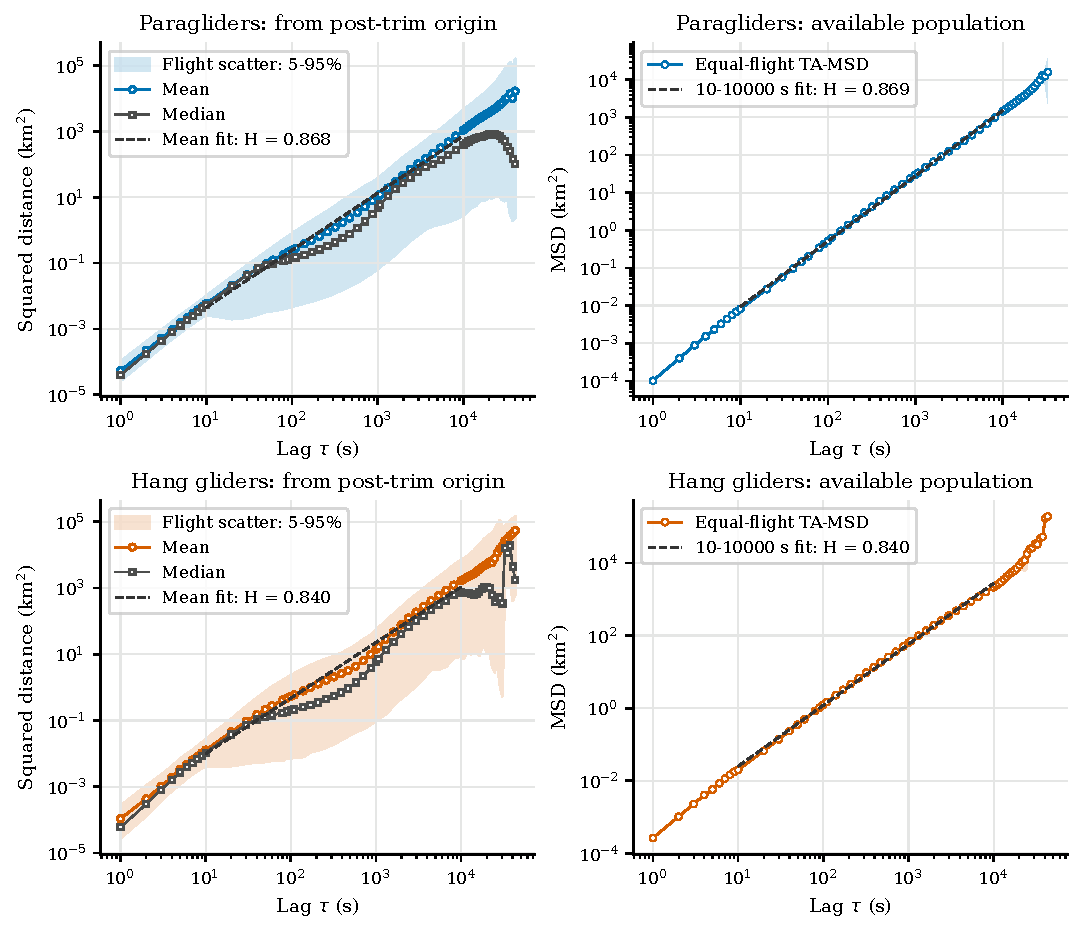
\includegraphics[width=\textwidth]{generated/ch3_transport_general.pdf}
 \caption{General horizontal transport. Left: squared distance from the post-trim
 origin, with equal-flight mean, median and the empirical 5--95\% flight range.
 Right: equal-flight TA-MSD over the population available at each lag, with
 pointwise 90\% cluster-bootstrap intervals and a log--log fit over
 \ChThreeGeneralFitLagMin--\ChThreeGeneralFitLagMax{} s (evaluated lags:
 \ChThreeGeneralFitLagMin--\ChThreeGeneralLastFitLag{} s). Native short-lag support
 differs from common-grid support.}
 \label{fig:fixed-general}
\end{figure}

\begin{figure}[p]
 \centering
 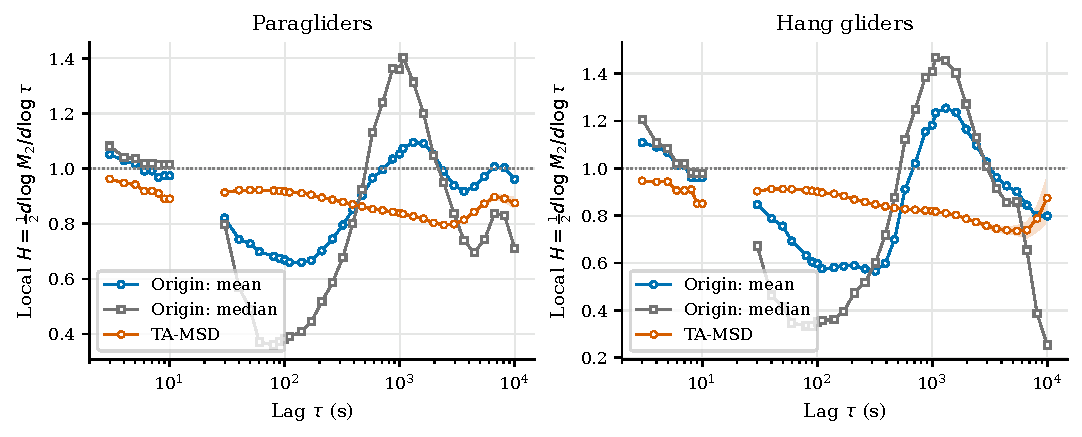
\includegraphics[width=\textwidth]{generated/ch3_transport_general_slopes.pdf}
 \caption{Local slopes of the general curves. The origin-distance mean and median
 have no confidence band here; the TA-MSD band is obtained by refitting bootstrap
 curves. The horizontal coordinate is elapsed time $t$ from trimming for the
 origin-distance curves and lag $\tau$ for the TA-MSD. The dotted reference is
 ballistic growth, $H=1$.}
 \label{fig:fixed-general-slopes}
\end{figure}
We summarise the growth of the TA-MSD by an ordinary-least-squares linear fit of
$\log_{10}M_2$ against $\log_{10}\tau$. A power law $M_2\propto\tau^{2H}$ has slope
$2H$ in this plane, so $H$ is half the fitted slope.
Here $H$ denotes an effective growth exponent: its identification with a process's
self-similarity exponent is tested in the experimental Section~\ref{sec:fixed-scaling}.  The
interval for $H$ comes from repeating the fit on the TA-MSD recomputed for each
bootstrap replicate, a resampling of site--day groups described in the paragraph
``\nameref{par:fixed-uncertainty}'' below.
The fits to the TA-MSD of the available population (Figure~\ref{fig:fixed-general},
right) are requested over
\ChThreeGeneralFitLagMin--\ChThreeGeneralFitLagMax{} s but the last lag of the grid inside
that range is \ChThreeGeneralLastFitLag{} s, so they span
\ChThreeGeneralFitLagMin--\ChThreeGeneralLastFitLag{} s.
In the right panels of Figure~\ref{fig:fixed-general}, the TA-MSD over the fitted lags
lies close to a straight line in logarithmic scale. Figure~\ref{fig:fixed-general-residuals}
shows the fit residuals: they
fall on both sides of zero over the whole fitted range, and their RMS say that a
typical measured value lies within a factor \ChThreeParaGeneralRmsRatio{} and
\ChThreeHangGeneralRmsRatio{} of the fitted line, respectively for paragliders and hang gliders.
Such ratios, close to
unity over a curve that grows by about six decades, combined with the fact that the residuals
are evenly distributed above and below the fitted curve, make the line an adequate
description of the measured growth. The residuals are nevertheless not scattered at random.
In fact, they change sign three times as
the lag grows, so the departure from a single power law is a smooth curvature, largest
at the longest lags where the contributing population has shrunk most
(Table~\ref{tab:fixed-support}). The fit therefore summarises the growth as one
effective exponent, and the local exponent below (Figure~\ref{fig:fixed-general-slopes})
shows how the slope varies with lag.

\begin{figure}[htbp]
 \centering
 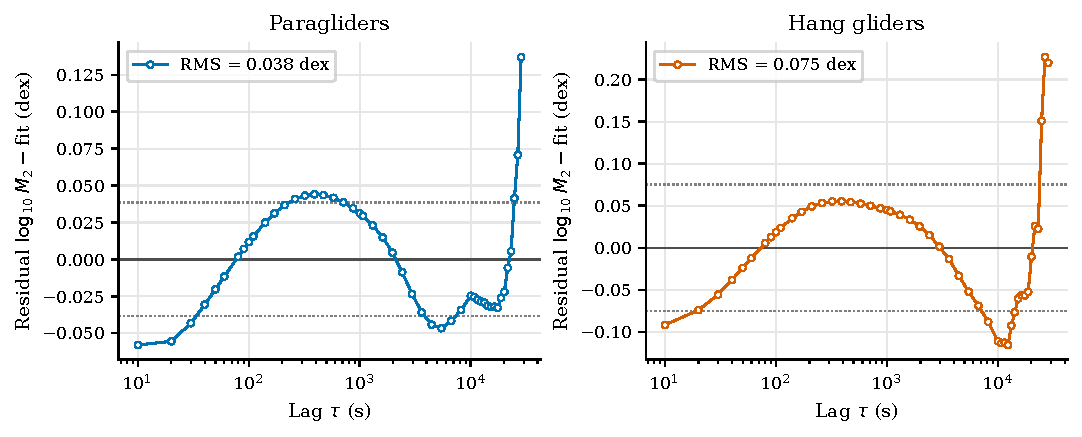
\includegraphics[width=\textwidth]{generated/ch3_transport_general_residuals.pdf}
 \caption{Residuals of the log--log fit of the general TA-MSD at the fitted lags, in dex:
 $\log_{10}M_2$ minus the fitted line. A residual of $r$ dex means the measured curve
 sits a factor $10^{r}$ from the line, so $0$ dex is a point lying on it. Dotted lines
 mark plus and minus the RMS residual.}
 \label{fig:fixed-general-residuals}
\end{figure}

The available-population fits give, with 90\% bootstrap intervals in brackets:
\begin{itemize}
      \item paragliders: $H=\ChThreeParaGeneralHurst$ over
      \ChThreeGeneralFitLagMin--\ChThreeGeneralLastFitLag{} s;
      \item hang gliders: $H=\ChThreeHangGeneralHurst$ over the same lags.
\end{itemize}

Since the flights contributing at each lag
change as $\tau$ grows (Table~\ref{tab:fixed-support}), these values summarise the
growth of a curve whose population shrinks with lag.

\begin{table}[htbp]
 \centering\small
 \begin{tabular}{lrrr}
\toprule
Discipline & Lag (s) & TA-MSD flights & Origin-distance flights\\
\midrule
Paragliders & 10 & 155,085 & 152,771\\
Paragliders & 100 & 155,044 & 155,117\\
Paragliders & 1000 & 154,482 & 155,250\\
Paragliders & 10000 & 46,273 & 72,160\\
Paragliders & 32690 & 27 & 1,237\\
Hang gliders & 10 & 6,060 & 5,330\\
Hang gliders & 100 & 6,060 & 6,059\\
Hang gliders & 1000 & 6,044 & 6,070\\
Hang gliders & 10000 & 2,326 & 3,480\\
Hang gliders & 43200 & 1 & 3\\
\bottomrule
\end{tabular}

 \caption{Number of contributing flights in the general curves. The last row for
 each discipline is the largest evaluated lag with TA-MSD support. The origin-distance
 curve uses elapsed time; the TA-MSD requires a within-segment lag no larger than
 $0.8T_s$. Their support sets therefore differ. Early origin-distance support can increase
 when elapsed time exceeds an initial excluded interval or resolves a coarse cadence.}
 \label{tab:fixed-support}
\end{table}

To describe how growth varies with lag, we also estimate the local exponent
\begin{equation}
 H_{\rm loc}(\tau)=\frac12\frac{d\log M_2(\tau)}{d\log\tau}.
 \label{eq:fixed-local-h}
\end{equation}
At each lag, we fit a straight line by ordinary least squares to the log--log curve
within $\pm0.25$ decades and take half its slope. At least three lags are required.
For sparse interior windows in the general curves, we use the three nearest lags
in logarithmic distance; this fallback requires at least two available grid lags
on each side of the target. Otherwise, windows with fewer than three lags are
left unestimated.

The TA-MSD band in Figure~\ref{fig:fixed-general-slopes} is the pointwise 5--95\%
range obtained by repeating the local fits on the same bootstrap curves.
The origin-distance mean and median use the same method with elapsed time $t$
in place of lag $\tau$.

Figures~\ref{fig:fixed-general} and~\ref{fig:fixed-general-slopes} show two linked
features of the origin-distance curves. After the approximately ballistic regime
at $t\lesssim10$ s, the mean rises visibly above the median, with a marked
separation at $t\sim10^2$--$10^3$ s. The mean's local slopes reach minima at \ChThreeParaLocalMinLag{} s
($H_{\rm loc}=\ChThreeParaLocalMinH$) for paragliders and \ChThreeHangLocalMinLag{} s
($H_{\rm loc}=\ChThreeHangLocalMinH$) for hang gliders within 20--2000 s, then recover
towards $H_{\rm loc}\simeq1$ around 600--700 s.


A possible physical explanation is the asynchronous alternation of gliding,
search and climb. At the same elapsed time, some pilots glide while others search
for lift or circle in a thermal, making less net horizontal progress. At short
elapsed times, an episode of searching or lifting lasting a few hundred seconds can greatly reduce the
displacement relative to a flight that keeps gliding. The latter pulls the mean
above the median, especially because displacement is squared. Meanwhile, the
slow horizontal progress of flights in search and climb lowers the growth rates,
with a stronger dip in the median's $H_{\rm loc}$.

The duration distributions in Vilpellet et al.~\cite[Fig.~4f,i]{vilpellet2026}
support this timescale: search times and climb times have survival probabilities that remain of order $10^{-3}$ at
durations of several hundred seconds. An archive with many thousands of flights
can therefore contain several such long events alongside much shorter ones.

Search and climb continue throughout the flight, at different times for different
pilots. At $t\sim10^3$--$10^4$ s, however, many flights have already reached much
larger distances from the origin. The extra displacement gained by gliding rather
than searching or climbing during one interval of $10^2$--$10^3$ s can then be
smaller relative to that distance, and so have a smaller relative effect on
squared distance. The same alternation of phases can thus produce a weaker contrast between
flights at long elapsed times. This is consistent with the recovery of the local
exponents and the narrowing of the early mean--median gap, even though the phases
remain asynchronous.

\paragraph{Uncertainty.}\label{par:fixed-uncertainty} The shading around the origin-distance curves of
Figure~\ref{fig:fixed-general} is the empirical 5--95\% range across flights, a
measure of scatter among flights. Every other shaded band in this chapter is a
pointwise 90\% bootstrap interval: the interval is constructed separately at each
lag, with nominal 90\% coverage at that lag, rather than simultaneous 90\% coverage
of the entire curve. Flights are grouped by
catalogue take-off site (the one declared in the FFVL catalogue metadata
(Section~\ref{sec:catalog}, Table~\ref{tab:catalogfields})) and calendar date, retaining dependence within each site--day.
Missing keys give singleton groups.
A \emph{replicate} is one resampled version of the archive.\\\\
Writing $G$ for the number of site--day groups in the eligible archive, we construct
$B=1000$ replicates once, before evaluating the MSD at the different lags. Each
replicate draws $G$ groups with replacement and retains all flights in each selected
group. Thus $G$ counts group selections, including repetitions; the number of
distinct groups and the total number of flights can vary between replicates.

At each lag $\tau$, we evaluate the MSD using only the flights in that replicate
that have admissible increments at $\tau$, namely those in $\mathcal C(\tau)$.
As $\tau$ increases, flights with insufficient segment duration cease to contribute,
but the original group draws remain fixed: no replacement flights or groups are
drawn. A group selected twice still counts each of its contributing flights twice;
if none of its flights supports that lag, it contributes nothing there.
The MSD is divided by the number of contributing flights in that replicate at that
lag, counting repetitions. This count can vary both between replicates and with
$\tau$.
An analysis of a sub-population, such as a duration cohort, reuses the same draws
and keeps only the flights that belong to it.
Let $g(f)$ be the group of flight $f$, and $c^{(b)}_g$ the number of times group $g$ is
drawn in replicate $b$. The replicate replaces the equal weight $1/N(\tau)$ of
Eq.~\eqref{eq:fixed-msd} by a weight proportional to the multiplicity of the flight's
group:
\begin{equation}
 M_2^{(b)}(\tau)=\frac{1}{N^{(b)}(\tau)}
 \sum_{f\in\mathcal C(\tau)}c^{(b)}_{g(f)}\,m_f(\tau),
 \qquad
 N^{(b)}(\tau)=\sum_{f\in\mathcal C(\tau)}c^{(b)}_{g(f)}.
 \label{eq:fixed-bootstrap}
\end{equation}
Setting every $c^{(b)}_g=1$ recovers Eq.~\eqref{eq:fixed-msd}. The multiplicities
$c^{(b)}_g$ have no lag dependence; the contributing set $\mathcal C(\tau)$ and
normalisation $N^{(b)}(\tau)$ do. Each of the 1000 replicates uses its own group draw
consistently across lags, observables and cohorts. For a comparison between two
cohorts, we subtract their estimates within each replicate, producing 1000
differences, one for each $b=1,\ldots,1000$. Their 5th and 95th percentiles give the
interval for the difference, retaining the sampling fluctuations shared by the
two cohorts. The point estimate itself is the difference between the estimates
from the original archive. We use this procedure for the duration-cohort contrasts
in Section~\ref{sec:fixed-population} and the open--closed circuit contrasts in
Section~\ref{sec:conditional-circuit}.
Quantiles and ratios are likewise recalculated within each replicate, and each fit
uses points from that replicate's curve, preserving the dependence between lags.
For an estimate $\widehat\theta$,
the 5th and 95th percentiles of the bootstrap replicates $\{\widehat\theta^{(b)}\}_{b=1}^{1000}$ give a pointwise 90\% confidence interval
\begin{equation}
 I_{90}(\theta)=
 \left[\operatorname{perc}_{5}\{\widehat\theta^{(b)}\}_{b=1}^{1000},\,
       \operatorname{perc}_{95}\{\widehat\theta^{(b)}\}_{b=1}^{1000}\right].
 \label{eq:fixed-ci}
\end{equation}
Percentiles are linearly interpolated between ordered estimates, excluding any
replicate with no contributing flights at the lag considered.\\\\

Cluster bootstrap requires many approximately independent groups and sufficiently
stable statistics~\cite{cameron_miller2015}; flights within a group need not be
independent. Table~\ref{tab:fixed-clusters} describes their spatial and temporal
separation. Nearby sites and successive days can share weather, so these distances
do not verify independence; the paragraph below checks MSD and fitted-exponent errors using geographic,
altitude and seasonal groups. Residual dependence may make the bands
too narrow; upload selection also limits inference to the population represented
by the archive. General TA-MSD bands are omitted below 20 contributing groups.

The statistical validity of these intervals is therefore not established at this
stage. Independence between site--day groups is assumed and has never been verified,
and the size of the groups makes the assumption doubtful: their median size is one
flight, the 95th percentile is five flights for paragliders and three for hang
gliders, and even the largest group holds 47 and 13 flights
(Table~\ref{tab:fixed-clusters}). A partition this fine absorbs little of the
dependence it was introduced to capture. Flights that share one weather episode
across neighbouring sites, or across consecutive days at the same site, fall into
different groups and are resampled as if they carried independent information. The
groups are then probably not independent, and Eq.~\eqref{eq:fixed-ci} probably
understates the true uncertainty, so every band reported in this chapter should be
read as a lower bound on the spread. The open question is whether bootstrap groups
coarse enough to be approximately independent can be built at all. The paragraph
below is a first attempt at it and has not answered it yet, which is why it is
typeset in red.

\begin{table}[htbp]
 \centering\small\setlength{\tabcolsep}{4pt}
 For paragliders, the main cohort spans 3,424 catalogue sites and 3,642 dates; group size has median 1, the 95th percentile 5, and the largest group 47 (0.10\% of flights). Where another site is represented on the same day (24,509 of 25,682 groups), its nearest distance has median 11.2 km and 10--90\% range 0.04--173 km. The gap from the previous observed date at the same site is 19 days (10--90\%: 1--429; 22,258 comparisons). Missing group keys affect 0 main-cohort flights.

For hang gliders, the main cohort spans 284 catalogue sites and 1,017 dates; group size has median 1, the 95th percentile 3, and the largest group 13 (0.56\% of flights). Where another site is represented on the same day (1,147 of 1,768 groups), its nearest distance has median 24.7 km and 10--90\% range 0.04--338 km. The gap from the previous observed date at the same site is 18 days (10--90\%: 1--382; 1,484 comparisons). Missing group keys affect 0 main-cohort flights.

 \caption{Site--day diagnostics in the main cohort. Distances refer to the nearest
 other catalogue site represented on the same date; time gaps refer to the previous
 observed date at the same site. Distances and time gaps are reported as median
 [10th, 90th percentile].
 Cohort group counts are in Table~\ref{tab:fixed-cohorts}.}
 \label{tab:fixed-clusters}
\end{table}

\Needspace{12\baselineskip}
\begin{wipblock}
\paragraph{Reliability of bootstrap uncertainty estimates (work in progress, not
working).}
\label{sec:fixed-bootstrap-reliability}

This paragraph is a working draft and no conclusion in it is settled. The grouping
tried here does not yet produce approximately independent bootstrap groups, so its
intervals validate nothing and its numbers are reported only to record where the
attempt stands.

We repeat the uncertainty check with groups defined by a fixed geographic cell,
launch-altitude class and month of the year, pooling all years. Thus July flights
from different years share a group when their initial positions lie in the same
cell and altitude class. The grid is independent of the observed sites: each
initial position belongs to one half-open $50\times50$ km square in its WGS84 UTM
zone, with sides measured in projected metres. Cells are clipped at zone and
hemisphere boundaries. The four altitude classes (plains, hills, low and high
mountains) retain the existing thresholds of 300, 800 and 1500 m; they are a proxy
for launch orography. This construction groups geographical and seasonal context,
not necessarily a common weather episode.

All main-cohort flights and their equal-flight weights are retained. We draw 1000
bootstrap replicates, paired across lags, and repeat with two seeds. The archived
site--day bootstrap provides the reference. Table~\ref{tab:fixed-grid-groups}
compares group composition. Singleton groups remain, but contain only
\ChThreeParaGridSingletonFlightPct\% of paraglider flights and
\ChThreeHangGridSingletonFlightPct\% of hang-glider flights. The standard error of
$H$ is \ChThreeParaGridHFactor{} and \ChThreeHangGridHFactor{} times the site--day
value, respectively; point estimates are unchanged.

\begin{table}[htbp]
 \centering\small\setlength{\tabcolsep}{4pt}
 \begin{tabular}{lrrrrr}
\toprule
 & Site--day & Grid & Median size & Singletons (\%) & Max. share (\%) \\
\midrule
Paragliders & 25682 & 1901 & 3 & 33.5 & 4.4 \\
Hang gliders & 1768 & 267 & 2 & 43.4 & 13.4 \\
\bottomrule
\end{tabular}

 \caption{Bootstrap groups of the main cohort before and after cell--altitude--month
 grouping. ``Before'' are the site--day groups that resample every other interval in
 this chapter; ``after'' are the alternative groups introduced in this check, used only
 here. Median size is the number of flights per new group. Singletons are expressed as
 a percentage of new groups; maximum share is the largest group's percentage of
 cohort flights. All years are pooled within each month.}
 \label{tab:fixed-grid-groups}
\end{table}

We test sensitivity using 10, 25 and 50 km cells, shifting each grid by half a cell
along either or both axes. Separately, we merge two or three adjacent months and
shift the seasonal boundaries, retaining 50 km cells and the altitude classes
(Fig.~\ref{fig:fixed-bootstrap-reliability}). These are alternative resampling
partitions, not exclusions of flights.

\begin{figure}[htbp]
 \centering
 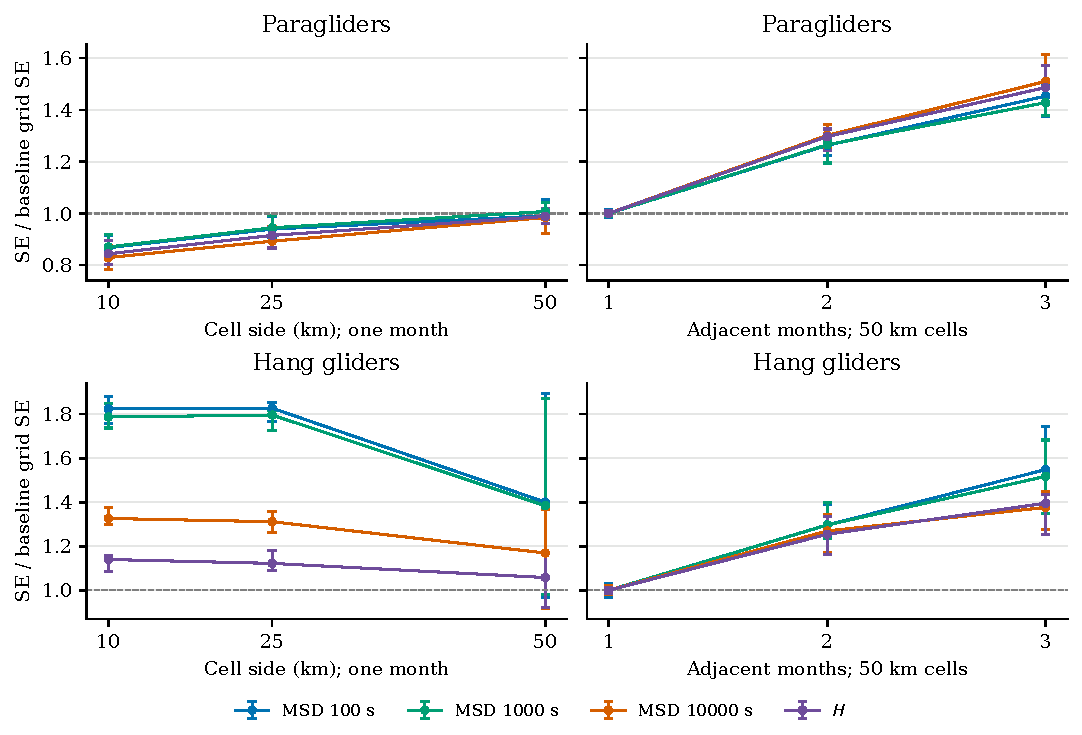
\includegraphics[width=\textwidth]{generated/ch3_transport_grid_bootstrap.pdf}
 \caption{Standard errors relative to the unshifted 50 km, one-month grid baseline.
 Left: cell size and boundary shifts. Right: adjacent-month unions with seasonal
 boundary shifts. Markers are medians and bars span minima and maxima across
 partitions and two seeds; they are not confidence intervals. Altitude classes
 remain separate, and all years are pooled.}
 \label{fig:fixed-bootstrap-reliability}
\end{figure}

The uncertainty has not stabilised across these choices. Merging three months
multiplies the median standard error of $H$ by \ChThreeParaGridHThreeMonths{} for
paragliders and \ChThreeHangGridHThreeMonths{} for hang gliders. For the latter,
shifting the 50 km grid gives MSD errors at 1000 s ranging from
\ChThreeHangGridMsdShiftRange{} times the unshifted value. Larger groups therefore
do not by themselves validate independence or interval coverage. Neighbouring
cells, months and altitude classes can still share conditions, while persistent
geographical differences can also affect the comparison~\cite{cameron_miller2015}.
The new intervals are conditional on this grouping; the archived site--day bands
elsewhere remain the reference and are not replaced by this MSD/$H$ check.
\end{wipblock}

\FloatBarrier

\subsection{Fixed population and the effect of duration selection}
\label{sec:fixed-population}

The general TA-MSD of Sec.~\ref{sec:fixed-general} averages over whichever flights
support each lag, so its population shrinks as $\tau$ grows: short flights and short
segments drop out one after another. The mix of circuit types and launch sites that
remains then changes with $\tau$, and a change in the slope of $M_2(\tau)$ cannot be
told apart from a change in the dynamics. Every statistic of the motion in the rest of
this chapter is therefore measured on one population that does not depend on $\tau$.
Such a population is limited by its shortest member: the longest lag it supports is
fixed by how long its segments are. Selecting only long segments gives more lags, and
loses flights. This subsection asks whether that selection changes the measured $H$
enough to matter, and chooses the cohort accordingly.

\paragraph{Cohorts.}
We select the segments once, using
\begin{equation}
 \tau_{\max}\leq0.8T_s,\qquad
 \mathcal C_{\tau_{\max}}=\{f:\exists s\in f,\ T_s\geq\tau_{\max}/0.8\},
 \label{eq:fixed-support}
\end{equation}
where $T_s$ is the segment's elapsed duration on the 10 s grid. The condition
$\tau_{\max}/T_s\leq0.8$ leaves $T_s-\tau_{\max}\geq0.2\,T_s$, one fifth of the
segment, for the origins at the largest lag. The threshold 0.8 fixes how many origins
remain there. For the main cohort, $\mathcal C_{10000}$, segments last at least
12500 s, so each supplies at least 251 origins on the 10 s grid at $\tau=10000$ s.
If a flight has segments of
14000 and 3000 s, only the first contributes, even at $\tau=10$ s. Flights and
selected segments therefore remain the same at every lag.

\paragraph{Weights.}
For the fixed cohort, $\mathcal I_f(\tau)$ and $n_f(\tau)$ refer only to its selected
segments, and Eq.~\eqref{eq:fixed-msd} still applies once $\mathcal C(\tau)$ and
$N(\tau)$ are replaced by the $\tau$-independent cohort and its size:
\begin{equation}
 m_f(\tau)=\frac1{n_f(\tau)}\sum_{i\in\mathcal I_f(\tau)}R_{fi}(\tau)^2,\qquad
 M_2(\tau)=\frac1N\sum_{f\in\mathcal C_{10000}}m_f(\tau),\qquad N=|\mathcal C_{10000}|.
 \label{eq:fixed-cohort-msd}
\end{equation}
Expanding the flight average $m_f(\tau)$ assigns every admissible origin of flight $f$
the same explicit weight
\begin{equation}
 w_f(\tau)=\frac{1}{Nn_f(\tau)},\qquad
 \sum_{i\in\mathcal I_f(\tau)}w_f(\tau)=\frac1N,
 \label{eq:fixed-weights}
\end{equation}
so that $M_2(\tau)=\sum_f\sum_{i}w_f(\tau)R_{fi}(\tau)^2$.\\
The same weights define the mean $\langle A\rangle_\tau=\sum_f\sum_{i}w_f(\tau)A_{fi}$ of any
per-origin quantity $A_{fi}$ (e.g.\ the signed displacement $\Delta x_{j,fi}(\tau)$
below), used from Eq.~\eqref{eq:fixed-kurtosis} onwards.

\begin{table}[htbp]
 \centering\small
 \begin{tabular}{llrrr}
\toprule
Discipline & $\tau_{\max}$ (s) & Flights & Segments & Groups\\
\midrule
Paragliders & 100 & 155,044 & 188,312 & 82,650\\
Paragliders & 1000 & 154,482 & 167,152 & 82,390\\
Paragliders & 10000 & 46,273 & 46,367 & 25,682\\
Hang gliders & 100 & 6,060 & 7,515 & 4,264\\
Hang gliders & 1000 & 6,044 & 6,610 & 4,253\\
Hang gliders & 10000 & 2,326 & 2,327 & 1,768\\
\bottomrule
\end{tabular}

 \caption{Nested duration cohorts and their site--day groups, the resampling
 units of Sec.~\ref{sec:fixed-general}. The nominal minimum durations
 $\tau_{\max}/0.8$ are 125, 1250 and 12500 s; since $T_s$ only takes multiples of
 10 s, the effective cutoffs are 130, 1250 and 12500 s.}
 \label{tab:fixed-cohorts}
\end{table}

\paragraph{Effect of the selection on $H$.}
We assess duration selection with the nested cohorts $\mathcal C_{100}$ and
$\mathcal C_{1000}$. They contain the main cohort's segments, additional shorter
segments of its flights, and additional flights. Selecting long segments also changes
who is in the sample. For example, the declared circuit class, open-distance flights
against closed routes such as triangles and out-and-return flights
(Sec.~\ref{sec:fixed-circuit}), shifts with the cohort: the share of closed routes
rises from
\ChThreeParaClosedFracStart\% in $\mathcal C_{100}$ to \ChThreeParaClosedFracMain\% in
$\mathcal C_{10000}$ for paragliders, and from \ChThreeHangClosedFracStart\% to
\ChThreeHangClosedFracMain\% for hang gliders.

Duration selection can also change the mix of launch environments and seasons.
The MSD and its fitted $H$ in $\mathcal C_{10000}$ could therefore differ from those
in $\mathcal C_{100}$, which retains almost the entire eligible archive. We compare
the cohorts to assess how much extending the accessible lag range changes the MSD
curve and its effective growth exponent.

We compare two cohorts $A$ and $B$ over the same lag interval. In each bootstrap
replicate, both use the same site--day group draw: we compare $H_A^{(1)}$ with
$H_B^{(1)}$, $H_A^{(2)}$ with $H_B^{(2)}$, and so on. This gives 1000 paired
differences,
\[
 \Delta H^{(b)}=H_A^{(b)}-H_B^{(b)},\qquad b=1,\ldots,1000.
\]
The 5th and 95th percentiles of these differences form the interval in
Table~\ref{tab:fixed-cohort-fits}.

The cohorts share flights and site--day groups. Using the same draws gives each
shared group the same multiplicity in both cohorts, preserving the dependence
between their estimated exponents. When a draw shifts both exponents by similar
amounts in the same direction, those shifts largely cancel in $\Delta H$. Independent
draws would lose this cancellation and overestimate the uncertainty of the
difference.


\begin{figure}[htbp]
 \centering
 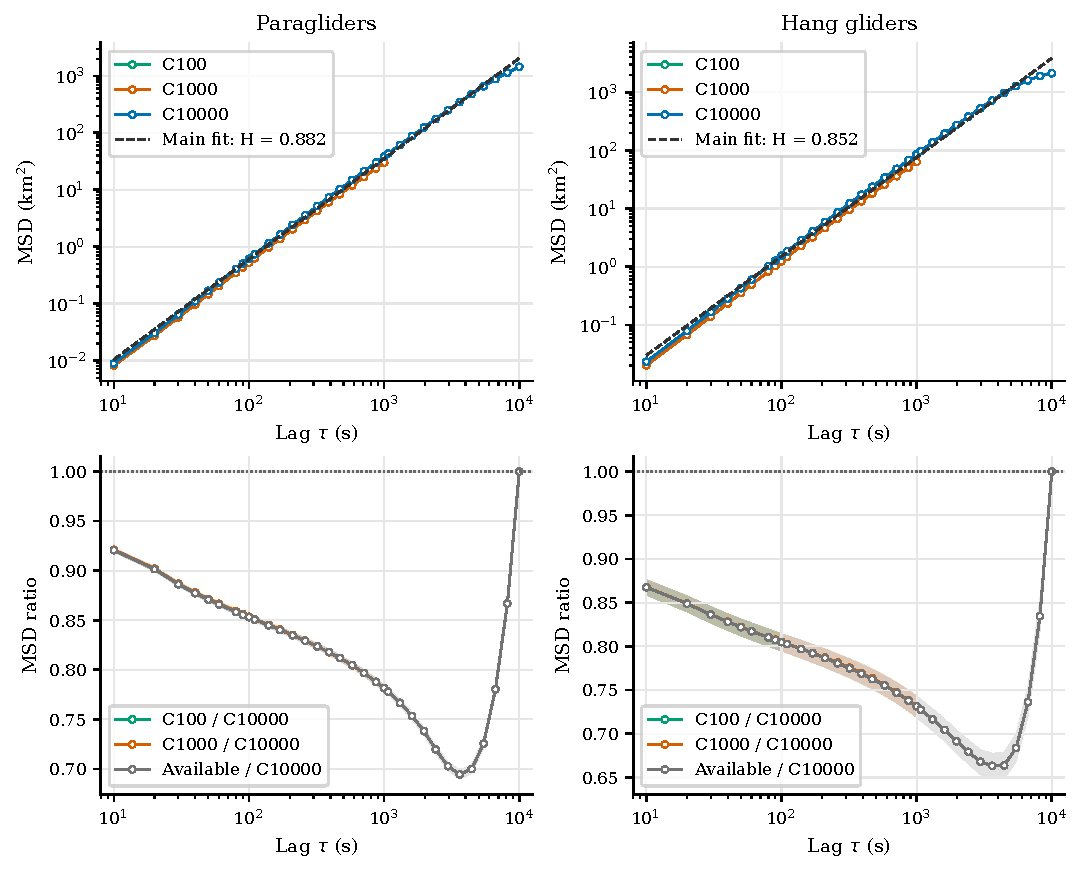
\includegraphics[width=\textwidth]{generated/ch3_transport_cohorts.pdf}
 \caption{Effect of duration selection. Top: MSD in the three nested cohorts, drawn
 lightest to darkest as $\mathcal C_{100}$, $\mathcal C_{1000}$, $\mathcal C_{10000}$;
 dashed lines fit the main cohort over 10--10000 s. The darkest curve is drawn on top
 and hides the lighter cohorts wherever they coincide, which is almost the whole
 visible range: the result below is that duration selection barely changes $H$.
 Bottom: effective $H$ with 90\% intervals, fitted over 10--100 s for all three
 cohorts and 10--1000 s for the two longer cohorts. Fits within each comparison use
 identical lag values.}
 \label{fig:fixed-cohorts}
\end{figure}
\begin{table}[htbp]
 \centering\small
 \begin{tabular}{lllr}
\toprule
Discipline & Fit range (s) & Contrast & $\Delta H$ [5--95\%]\\
\midrule
Paragliders & 10--100 & $H_{\mathcal C_{100}}-H_{\mathcal C_{1000}}$ & -0.00006 [-0.00009, -0.00004]\\
Paragliders & 10--100 & $H_{\mathcal C_{100}}-H_{\mathcal C_{10000}}$ & -0.01687 [-0.01712, -0.01660]\\
Paragliders & 10--100 & $H_{\mathcal C_{1000}}-H_{\mathcal C_{10000}}$ & -0.01680 [-0.01705, -0.01654]\\
Paragliders & 10--1000 & $H_{\mathcal C_{1000}}-H_{\mathcal C_{10000}}$ & -0.01703 [-0.01733, -0.01674]\\
Hang gliders & 10--100 & $H_{\mathcal C_{100}}-H_{\mathcal C_{1000}}$ & -0.00002 [-0.00013, 0.00011]\\
Hang gliders & 10--100 & $H_{\mathcal C_{100}}-H_{\mathcal C_{10000}}$ & -0.01646 [-0.01748, -0.01552]\\
Hang gliders & 10--100 & $H_{\mathcal C_{1000}}-H_{\mathcal C_{10000}}$ & -0.01644 [-0.01746, -0.01550]\\
Hang gliders & 10--1000 & $H_{\mathcal C_{1000}}-H_{\mathcal C_{10000}}$ & -0.01771 [-0.01879, -0.01668]\\
\bottomrule
\end{tabular}

 \caption{Paired differences of the cohort exponents, with 5--95\% bootstrap intervals.
 Each comparison uses identical lags and draws. The $\mathcal C_{100}$--$\mathcal C_{1000}$
 shift is negligible in magnitude ($|\Delta H|<10^{-4}$), although statistically
 resolved for paragliders. Contrasts with $\mathcal C_{10000}$ exclude zero and
 represent a larger, but still small, shift of about 2\% in $H$.}
 \label{tab:fixed-cohort-fits}
\end{table}
\paragraph{Result.}
On 10--100 s, $\mathcal C_{100}$ and $\mathcal C_{1000}$ differ in $H$ by less than
$10^{-4}$ in both disciplines. The paired interval resolves this tiny difference for
paragliders; for hang gliders it includes zero. The two cohorts share
\ChThreeParaCohortOverlapPct\% (paragliders) and \ChThreeHangCohortOverlapPct\% (hang
gliders) of their flights, so in each replicate their exponents move together and
their difference has a very narrow interval.\\
For the present analysis, we regard the two cohorts as having
practically the same $H$ on this lag range.\\

The main cohort behaves differently. Its effective exponent is larger than that of
every broader cohort, in both fit intervals and both disciplines, and every one of
these paired differences excludes zero. The difference between the main cohort and a
broader one lies between \ChThreeCohortShiftMin{} and \ChThreeCohortShiftMax{} in $H$,
which is \ChThreeCohortBiasMinPct--\ChThreeCohortBiasMaxPct\% of the exponent itself.

Two candidate explanations concern who, and under what conditions, flies long
enough to enter the main cohort. One is that sustaining a segment of 12500 s,
nearly four hours, selects more experienced pilots. Vilpellet et al.~\cite{vilpellet2026} find that,
taking the class of the glider as a proxy for experience, the MSD exponent of the
search phase grows with experience, and interpret this as skill enhancing the
ability to probe, interpret and exploit atmospheric cues. Experienced pilots may
therefore locate and exploit thermals more efficiently, cutting the time spent
searching rather than gliding, which raises $H$. The other is that it
selects better flying days, where stronger or more reliable lift shortens that same
search time for any pilot.

We accept this small bias and adopt $\mathcal C_{10000}$ for every analysis below that
requires a fixed population. A shift of about 2\% in $H$ is small beside what the cohort
provides: a population that stays the same over three decades of lag, 10--10000 s,
against two for $\mathcal C_{1000}$ and one for $\mathcal C_{100}$.



\section{Conditional mean-square displacement}
\label{sec:fixed-circuit}

We examine how MSD amplitude and its effective growth exponent $H$ vary with
three recorded characteristics:
\begin{itemize}
 \item \emph{Circuit type}: open distance flights versus closed routes, then
 the four declared types of closed route.
 \item \emph{Launch environment}: initial altitude as a proxy for plains,
 hills and mountains, followed by regional comparisons within these settings.
 \item \emph{Equipment}: wing class as a proxy for pilot experience.
\end{itemize}
\emph{Marginal comparisons} pool the other characteristics; \emph{stratified
comparisons} keep a selected category fixed, for example comparing circuits
within each altitude class. This tests whether a contrast survives
stratification and whether its magnitude depends on the other factor.
These observational comparisons differ from a \emph{one-factor-at-a-time}
(OFAT) experiment, which varies one input while holding the others at fixed
settings and does not estimate interactions~\cite{nist_ofat}.
Here the remaining flight conditions can still differ between groups.

\Needspace{8\baselineskip}
We use the larger paraglider population to retain support after stratification.
Every group $\mathcal C_g$ belongs to the fixed cohort $\mathcal C_{10000}$,
with the same retained segments throughout $10\leq\tau\leq10000$ s:
\begin{equation}
 M_{2,g}(\tau)=\frac{1}{N_g}\sum_{f\in\mathcal C_g}m_f(\tau),
 \qquad N_g=|\mathcal C_g|,
 \qquad M_{2,g}(\tau)\propto\tau^{2H_g},
 \label{eq:conditional-msd}
\end{equation}
Differences in $H$ use the same 1000 site--day bootstrap draws across groups
and lags, paired as in Section~\ref{sec:fixed-population}. The intervals retain
the limitations discussed in Section~\ref{sec:fixed-bootstrap-reliability}.

\subsection{Declared circuit: the marginal comparison}
\label{sec:conditional-circuit}

The catalogue separates open distance flights from closed routes, including
triangles and out-and-return flights. The declaration describes the objective;
the recorded, trimmed trajectory need not end at its starting point.

We first pool all initial altitudes within each circuit class. The fixed cohort contains
\ChThreeMainOpen{} open flights, \ChThreeMainClosed{} closed flights and
\ChThreeMainUnknown{} unclassified flights; the last group enters neither curve
in Figure~\ref{fig:conditional-circuit}.

\begin{figure}[htbp]
 \centering
 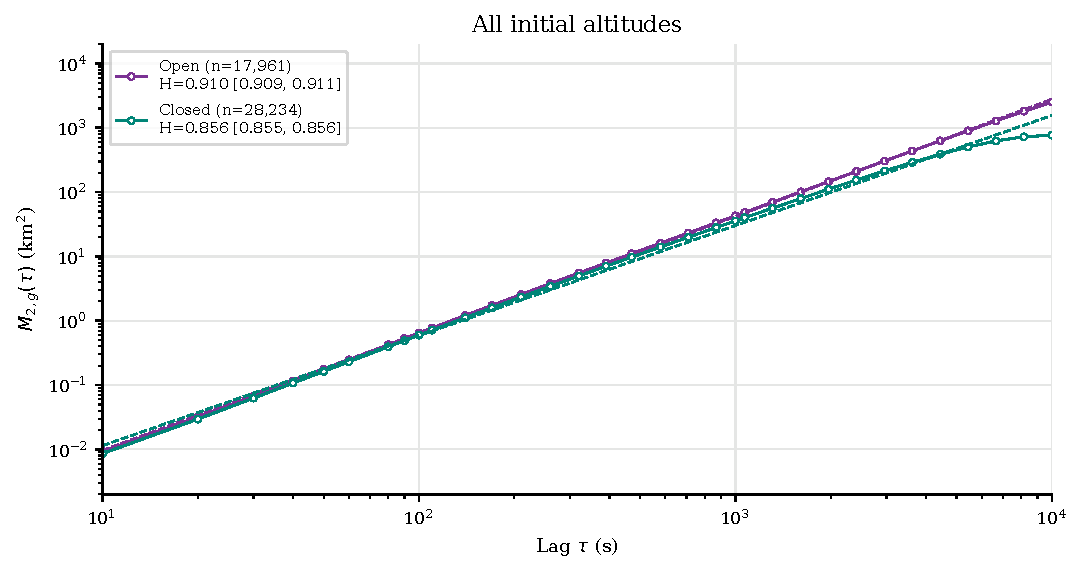
\includegraphics[width=\textwidth]{generated/ch3_conditional_circuit.pdf}
 \caption{Paraglider MSD by declared circuit, pooling initial altitudes. Solid
 curves join the equal-flight estimates; dashed lines are fits over 10--10000 s.}
 \label{fig:conditional-circuit}
\end{figure}

The open-route MSD grows faster and reaches a larger displacement amplitude at
long lags. Its effective exponent is \CondOpenH{}, compared with \CondClosedH{}
for closed routes. The paired difference $H_{\rm open}-H_{\rm closed}$ is
\CondOpenClosedDelta{}, so the separation is resolved under the adopted bootstrap.

\Needspace{9\baselineskip}
\paragraph{Circuit geometry and the separation of the curves.}
Closed routes must reverse part of their outward progress. Intervals spanning
turns or returns can therefore have smaller net displacements, consistent
with the slower long-lag MSD growth. The relevant timescale depends on the
route geometry and leg durations. For a flight of duration $T$ with equal
leg times, the first major turn occurs at $T/2$ for an out-and-return flight
and $T/3$ for a triangle. These are times along the route: even a short lag can straddle
a turn, because the MSD averages over starting points along each segment.
Section~\ref{sec:conditional-route} separates the declared closed route
types; their actual leg durations remain unmeasured.

\FloatBarrier
\subsection{Initial altitude, circuit composition and interaction}
\label{sec:conditional-orography}

The launch altitude $z_0$ defines four classes. It is the GNSS altitude of the first
fix of the trimmed track. The classes are: Plains ($z_0<300$ m), Hills
($300\leq z_0<800$ m), Low mountains ($800\leq z_0<1500$ m), and High mountains
($z_0\geq1500$ m).
All circuit declarations, including unclassified ones, contribute to
Figure~\ref{fig:conditional-altitude}. These are descriptive comparisons of the
flight populations launched in each setting, pooling their different circuit
compositions.

\begin{figure}[htbp]
 \centering
 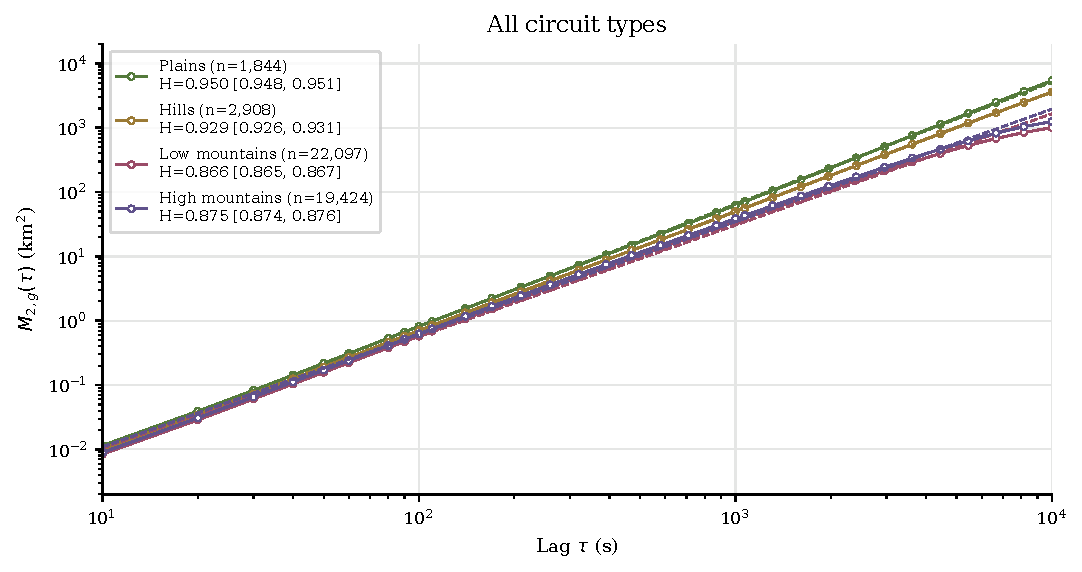
\includegraphics[width=\textwidth]{generated/ch3_conditional_altitude.pdf}
 \caption{Paraglider MSD by initial altitude, pooling circuit types and equipment.
 The four groups partition the fixed cohort. These marginal curves combine
 launch environment with unequal circuit proportions; they do not isolate
 an orographic effect.}
 \label{fig:conditional-altitude}
\end{figure}

Plains have the largest exponent, \CondAltZeroH{}, followed by Hills,
\CondAltOneH{}. Both exceed Low mountains, \CondAltTwoH{}, and High mountains,
\CondAltThreeH{}. The broad hierarchy is
\textbf{Plains $>$ Hills $>$ Mountains}, with High mountains slightly above
Low mountains.

The Plains--Low mountains difference is \CondAltZeroAltTwoDelta{}, about 10\%
of the smaller exponent. Interpreting this gap requires accounting for the
different circuit mixtures.

Open flights account for \ChThreeConditionalPlainsOpenPct\% of Plains and
\ChThreeConditionalHillsOpenPct\% of Hills, against
\ChThreeConditionalLowMountainsOpenPct\% and
\ChThreeConditionalHighMountainsOpenPct\% in the two mountain classes.
The lowland averages therefore give much greater flight weight to open routes.

\Needspace{8\baselineskip}
To explain the altitude curves, the relevant groups are the circuit types
\emph{within each altitude class}. Let $a$ denote that class and
$c\in\{\mathrm{open},\mathrm{closed},\mathrm{unclassified}\}$ its circuit
categories, omitting empty categories. With $N_{c,a}$ flights in each cell and $N_a=\sum_cN_{c,a}$,
the equal-flight estimator gives
\begin{equation}
 M_{2,a}(\tau)=\sum_c p_{c\mid a}M_{2,c,a}(\tau),
 \qquad p_{c\mid a}=\frac{N_{c,a}}{N_a},
 \qquad \sum_c p_{c\mid a}=1.
 \label{eq:fixed-mixture}
\end{equation}
The flight fractions $p_{c\mid a}$ stay fixed over the lag range. The fraction
of the class MSD supplied by circuit $c$ is
\begin{equation}
 w_{c\mid a}(\tau)=\frac{p_{c\mid a}M_{2,c,a}(\tau)}{M_{2,a}(\tau)},
 \qquad \sum_c w_{c\mid a}(\tau)=1.
 \label{eq:fixed-msd-share}
\end{equation}
In Figure~\ref{fig:conditional-circuit-weights}, shares sum to one
\emph{within each altitude class}, including its small unclassified component.

\begin{figure}[htbp]
 \centering
 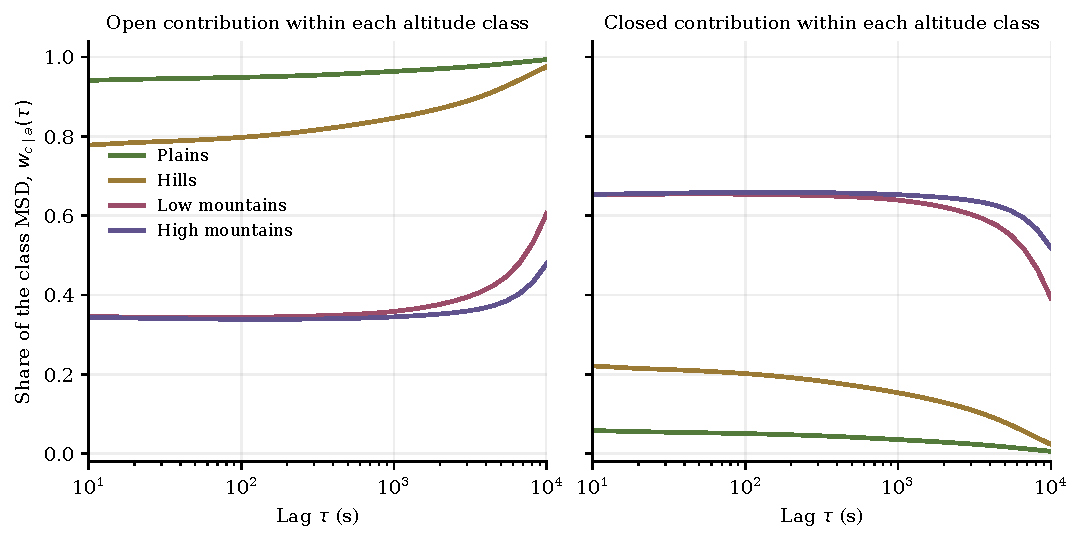
\includegraphics[width=\textwidth]{generated/ch3_conditional_circuit_weights.pdf}
 \caption{Circuit contributions to the MSD within each initial-altitude class.
 Left: $w_{\mathrm{open}\mid a}(\tau)$. Right:
 $w_{\mathrm{closed}\mid a}(\tau)$. The denominator is the full MSD of the
 indicated altitude class, including unclassified flights. Their unplotted
 contribution is at most \CircuitWeightUnknownMax\% over these curves.
 These are observed shares, without uncertainty bands.}
 \label{fig:conditional-circuit-weights}
\end{figure}

\begin{itemize}
 \item \textbf{A circuit's contribution depends on its MSD as well as its
 number of flights.}
 The larger open MSD amplifies the circuit imbalance in Plains and Hills.
 At $\tau=10000$ s, open routes supply
 \CircuitWeightPlainsOpenEnd\% and \CircuitWeightHillsOpenEnd\% of their
 respective class MSDs.
 In Low mountains, open flights are only
 \ChThreeConditionalLowMountainsOpenPct\% of the class, yet supply
 \CircuitWeightLowMountainsOpenEnd\% of its MSD at that lag: a minority of
 flights can contribute most of the MSD.

 \item \textbf{Circuit contributions change with lag and shape the pooled
 growth as well as its amplitude.}
 When open and closed MSDs grow at different rates, $w_{c\mid a}(\tau)$
 changes even though $p_{c\mid a}$ stays fixed. The open contribution rises
 towards long lags, particularly in the mountain classes. In High mountains,
 closed routes still supply \CircuitWeightHighMountainsClosedEnd\% at
 $10000$ s, whereas their contribution in Plains and Hills is already small.
 The exponent $H$ must therefore be fitted to the combined curve $M_{2,a}$;
 it is not generally a flight-count-weighted average of circuit exponents.
\end{itemize}

\paragraph{Circuit contrasts within altitude classes.}
Does the lowland advantage persist when circuit type is held fixed?
Figure~\ref{fig:fixed-task} crosses circuit type with altitude class;
Table~\ref{tab:fixed-task} reports counts, exponents and amplitudes.

\begin{figure}[htbp]
 \centering
 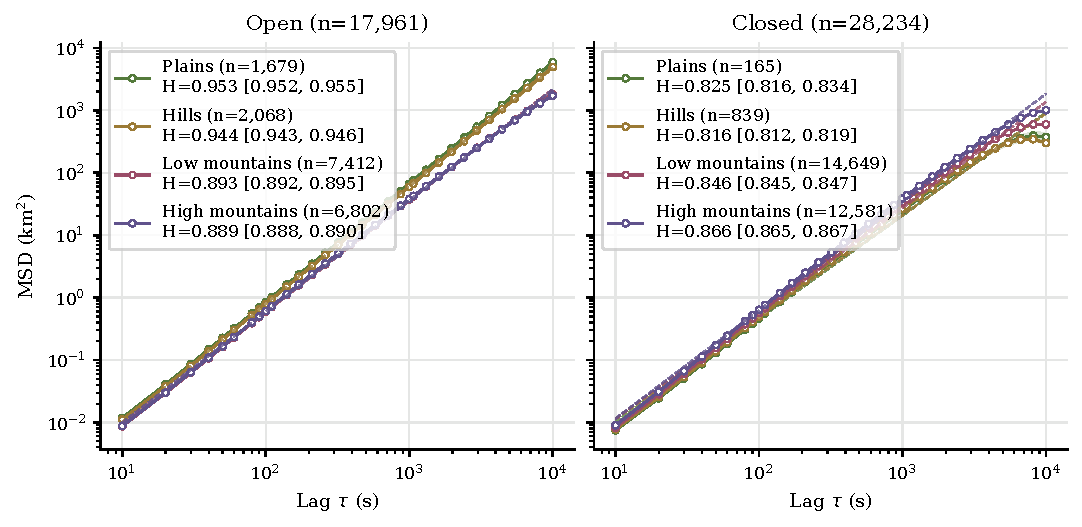
\includegraphics[width=\textwidth]{generated/ch3_transport_task_altitude.pdf}
 \caption{Paraglider transport by declared circuit and initial altitude, with fixed
 flights and segments throughout 10--10000 s. Markers give MSD estimates, shaded
 bands their pointwise 90\% intervals, and dashed lines the global log--log fits.
 Legends report the flight count and the fitted $H$ with its 90\% interval. The
 identical axes permit comparison of displacement amplitude and growth rate.}
 \label{fig:fixed-task}
\end{figure}
\begin{table}[htbp]
 \centering\footnotesize\setlength{\tabcolsep}{3.5pt}
 \begin{tabular}{llrrrr}
\toprule
Circuit & Initial altitude & $N$ & $G$ & $H$ [5--95\%] & $M_2(10^4)$ (km$^2$)\\
\midrule
Open & Plains & 1,679 & 1,140 & 0.953 [0.952, 0.955] & 5900\\
Open & Hills & 2,068 & 1,634 & 0.944 [0.943, 0.946] & 4920\\
Open & Low mountains & 7,412 & 5,255 & 0.893 [0.892, 0.895] & 1814\\
Open & High mountains & 6,802 & 4,794 & 0.889 [0.888, 0.890] & 1710\\
Closed & Plains & 165 & 157 & 0.825 [0.816, 0.834] & 372\\
Closed & Hills & 839 & 756 & 0.816 [0.812, 0.819] & 299\\
Closed & Low mountains & 14,649 & 7,954 & 0.846 [0.845, 0.847] & 596\\
Closed & High mountains & 12,581 & 7,406 & 0.866 [0.865, 0.867] & 1001\\
\bottomrule
\end{tabular}

 \caption{Main-cohort flights $N$, site--day groups $G$, global effective exponents
 and displacement amplitude at 10000 s. Intervals come from the coupled cluster
 bootstrap. Even the smallest cell retains 165 flights from 157 groups.}
 \label{tab:fixed-task}
\end{table}

\begin{itemize}
 \item \textbf{Open routes have larger $H$ than closed routes in every
 altitude class.} The paired gaps (nominal 90\% intervals) are
 \ChThreeTaskGapPlains{} in Plains, \ChThreeTaskGapHills{} in Hills,
 \ChThreeTaskGapLow{} in Low mountains and \ChThreeTaskGapHigh{} in High mountains.
 All exclude zero, and the gap is smaller in mountains. The pooled circuit contrast therefore cannot
 be explained solely by the open population's greater lowland share.
 \item \textbf{The altitude ordering reverses with circuit type.}
 Both lowland classes have larger $H$ than either mountain class for open
 routes, but smaller $H$ for closed routes. The four lowland-minus-mountain
 differences lie between \ChThreeOpenAltShiftMin{} and
 \ChThreeOpenAltShiftMax{} for open routes; for closed routes they are
 negative, with magnitudes between \ChThreeClosedAltShiftMin{} and
 \ChThreeClosedAltShiftMax. All eight paired intervals exclude zero.
\end{itemize}
This reversal quantifies an interaction: the association between launch
environment and $H$ depends on circuit type. The predominance of open flights
contributes to the pooled lowland advantage, but does not explain away the
opposite within-circuit orderings. Mountain flights do not have smaller $H$
in general.

\paragraph{Interpreting circuit choice and terrain constraints.}
The return objective explains the expected sign of the circuit contrast;
terrain may explain why its magnitude changes. Sun-heated mountain slopes
can feed convection that rises along the slope and detaches near a crest;
thermal sources need not lie on the crest itself. Access to lift and terrain
clearance can channel both circuit types along slope-and-ridge
corridors~\cite[Chapters~9--10]{faa_glider2024}. In plains, smaller physical
barriers and separated heat sources, such as dry dark fields and paved
areas~\cite{ssa_lift_sources}, may leave more route choices.

\begin{itemize}
 \item \textbf{Open routes.} Following ridges and detouring between usable
 lift sources could interrupt outward progress, making mountain open
 flights less persistent than lowland open flights. This is consistent
 with their smaller $H$.
 \item \textbf{Closed routes.} The same terrain constraints can alter the
 size and timing of a return circuit. Longer legs or later returns could
 suppress MSD growth less over 10--10000 s, consistently with the larger
 mountain closed $H$. Terrain constraints alone do not guarantee that
 timing change; it must be tested against measured leg and return times.
\end{itemize}
Mountain open routes may thus appear ``less open'' and closed routes
``less closed'' in their finite-lag statistics: their fitted exponents are
closer, while their declared classes remain unchanged. This interpretation
is a hypothesis; the conditional orderings are measured, but the proposed
route changes have not yet been measured.

\paragraph{Observed climb locations in two viewer cells.}
Figure~\ref{fig:conditional-climb-planes} compares two selected
$5\times5$ km cells from the viewer: \textbf{High mountains \#2 (H2)}, in
the Aulp du Seuil area of the Chartreuse (Alps), and \textbf{Plains \#1 (P1)},
in Suisse Normande within the broad Channel Coast box. Their ranks refer to
all-time distinct crossing flights within each altitude band: 15,840 for H2
and 2,246 for P1.
P1 is inland and contains local slopes despite its low starting-altitude
classification.

The maps pool \textbf{all available dates and years, without a seasonal
restriction}, using the viewer's Vilpellet climb classification for both
disciplines, without the MSD cohort's duration restriction.
Each point marks a climb crossing at 100 or 600 m above a fixed cell
reference: 1756 m ASL for H2 and 185 m for P1, estimated from five and 1165
screened starts, respectively. The viewer labels this offset AGL; it is not
clearance above the terrain beneath each point.
Red lines trace approximate crests derived independently from the IGN RGE ALTI
terrain model~\cite{ign_rge_alti}: local transverse height maxima on a 25 m
grid, smoothed at 50 m. They include secondary ridges but are scale-dependent,
not an exhaustive inventory; their ground positions stay fixed at both heights.

\input{generated/ch3_thermal_panel_values}
\begin{figure}[p]
 \centering
 \begin{minipage}{.22\textwidth}\centering
  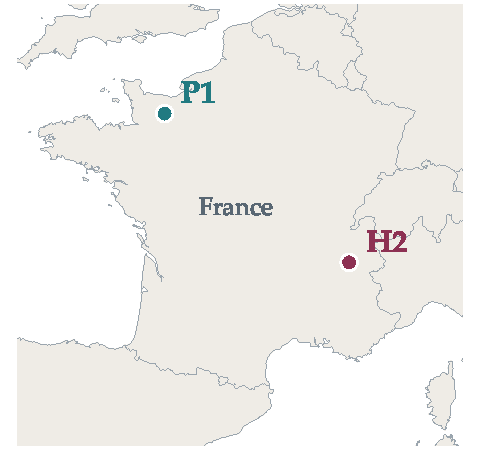
\includegraphics[width=\linewidth]{generated/ch3_thermal_cell_locator.pdf}
 \end{minipage}\hspace{.04\textwidth}
 \begin{minipage}{.64\textwidth}\small
  \textbf{H2: High mountains \#2, Chartreuse (Alps)}\\
  \textbf{P1: Plains \#1, Suisse Normande (Channel Coast)}\\[4pt]
  All available dates and years; no seasonal filter.\\
  Locator markers show cell centres, enlarged for visibility.
 \end{minipage}\\[6pt]
 \begin{minipage}{.43\textwidth}\centering\small
  \textbf{Alps: Chartreuse (H2)}\\[3pt]
  $z_{\mathrm{AGL}}=\ThermalLower$\\[3pt]
  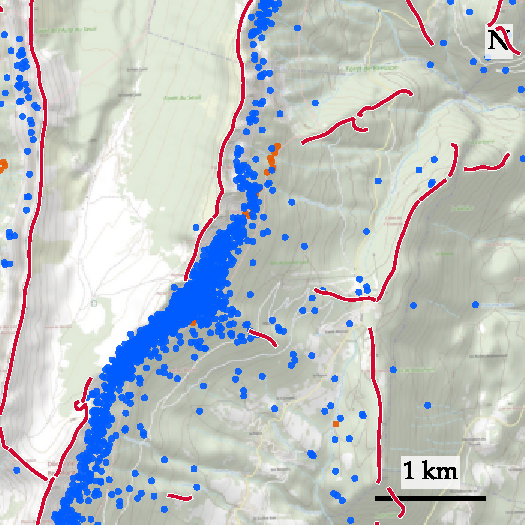
\includegraphics[width=\linewidth]{generated/ch3_thermal_mountain-low.pdf}\\
  \footnotesize\ThermalMountainLowCounts
 \end{minipage}\hfill
 \begin{minipage}{.43\textwidth}\centering\small
  \textbf{Alps: Chartreuse (H2)}\\[3pt]
  $z_{\mathrm{AGL}}=\ThermalUpper$\\[3pt]
  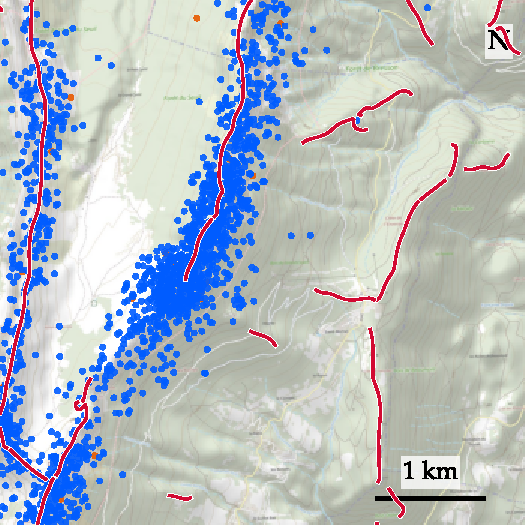
\includegraphics[width=\linewidth]{generated/ch3_thermal_mountain-high.pdf}\\
  \footnotesize\ThermalMountainHighCounts
 \end{minipage}\\[8pt]
 \begin{minipage}{.43\textwidth}\centering\small
  \textbf{Channel Coast: Suisse Normande (P1)}\\[3pt]
  $z_{\mathrm{AGL}}=\ThermalLower$\\[3pt]
  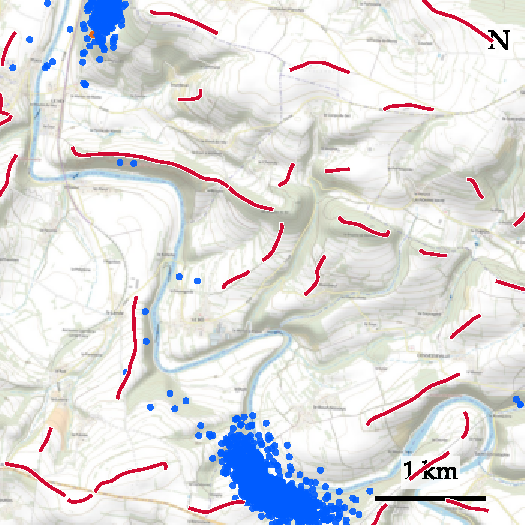
\includegraphics[width=\linewidth]{generated/ch3_thermal_plains-low.pdf}\\
  \footnotesize\ThermalPlainsLowCounts
 \end{minipage}\hfill
 \begin{minipage}{.43\textwidth}\centering\small
  \textbf{Channel Coast: Suisse Normande (P1)}\\[3pt]
  $z_{\mathrm{AGL}}=\ThermalUpper$\\[3pt]
  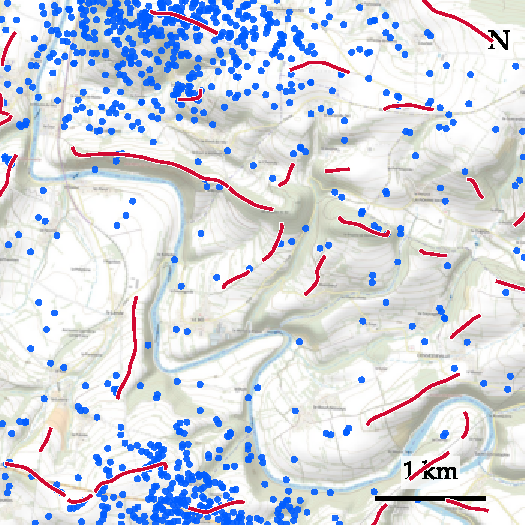
\includegraphics[width=\linewidth]{generated/ch3_thermal_plains-high.pdf}\\
  \footnotesize\ThermalPlainsHighCounts
 \end{minipage}
 \caption{Climb crossings in H2 and P1, at 100 and 600 m above each fixed cell
 reference, pooling all dates. Each pair covers the same $5\times5$ km
 footprint. Blue: paragliders; orange: hang gliders; red: approximate
 DEM-derived crests. Counts distinguish
 crossings from contributing flights, which differ between heights.
 Background: \copyright\ IGN/G\'eoplateforme, Plan IGN; terrain: RGE ALTI,
 Licence Ouverte 2.0.}
 \label{fig:conditional-climb-planes}
\end{figure}

\textbf{Climb locations spread out more visibly with height in P1 than in H2.}
At 100 m, P1 crossings cluster near local slopes; at 600 m, gliders cross
the plane while climbing over a much broader part of the cell. In H2, both
heights retain concentrations near the same terrain corridors, despite some
broadening at 600 m. The two main bands at 100 m follow mainly the outer
slopes of separate ridges---Lances de Malissard to the west and Aulp du
Seuil--Bellefont to the east of the Vallon de Marcieu---rather than opposite
slopes of a single central ridge. Thus gliders exploit
lift across a wider area aloft in P1, supporting greater spatial freedom
for route choices, while repeatedly using narrower terrain-associated
corridors in H2.

\textbf{Distributed sources and wind advection could jointly explain the
broader use of space aloft.} In an idealised steady plume, horizontal
advection $\boldsymbol{u}_h$ and upward air speed $w>0$ give
\[
 \Delta\boldsymbol{r}_h \simeq
 \frac{\boldsymbol{u}_h}{w}\,\Delta z.
\]
Drift therefore accumulates during ascent. Variation in wind direction,
speed or updraft strength across flights and days can broaden the pooled
crossing pattern with height. A common, constant wind and rise speed would
instead translate the source pattern; inclination alone does not imply
lift everywhere at a given height.

One possible mountain profile combines sheltered, heated slopes with
stronger winds above the crests: convection initially rises along or away
from the slope, then tilts more strongly aloft; strong shear can disrupt
it~\cite[Chapter~9]{faa_glider2024}. Exposed lowland sources may experience
advection from lower heights. These are possible conditions, not a general
wind hierarchy: valleys can also channel and accelerate
flow~\cite{schroeder_buck1970}. The maps do not establish either profile,
and the inland P1 cell cannot be assigned a coastal wind regime from its
regional label.

The maps show sampled climbs, including possible slope lift, rather than
tracked thermal centres. Different flights and weather support each height,
and low horizontal planes can intersect terrain. Their spatial contrast is
observed; attributing it to wind requires following the same climbs across
heights and matching wind profiles. Its contribution to $H$ and generality
across sites remain to be quantified.
\FloatBarrier
\subsection{Closed-route type and initial altitude}
\label{sec:conditional-route}

The closed class of Section~\ref{sec:conditional-circuit} pools four catalogue
labels: flat triangles, FAI triangles, quadrilaterals and out-and-return flights.
Together they make up the \ChThreeMainClosed{} closed flights of the fixed
cohort. The shortest side of an FAI triangle is at least 28\% of its
perimeter~\cite{ffvl_cfd_rules}. The flat-triangle label covers triangles scored
without this constraint, which can therefore be more elongated. An
out-and-return flight has a single turnpoint, and a quadrilateral has four legs.

The timescale argument of Section~\ref{sec:conditional-circuit} gives an
expectation. A route that reverses its outward progress later, or less often,
should suppress the long-lag MSD growth less. If route geometry controls $H$,
out-and-return flights should have the largest exponent and FAI triangles,
whose legs are the most balanced, the smallest, with flat triangles between
them.

Figure~\ref{fig:route-altitude} and Table~\ref{tab:route-altitude} cross the four
route types with the four initial-altitude classes of
Section~\ref{sec:conditional-orography}. The estimator, fit range and paired
bootstrap draws are those of Eq.~\eqref{eq:conditional-msd}. A cell receives an
interval only if it contains at least \RouteMinGroups{} site--day groups. The
quadrilateral and out-and-return cells of Plains and Hills hold between
\RouteOutAndReturnAltZeroN{} and \RouteQuadrilateralAltOneN{} flights each, so
they are reported by their counts only.

\begin{figure}[htbp]
 \centering
 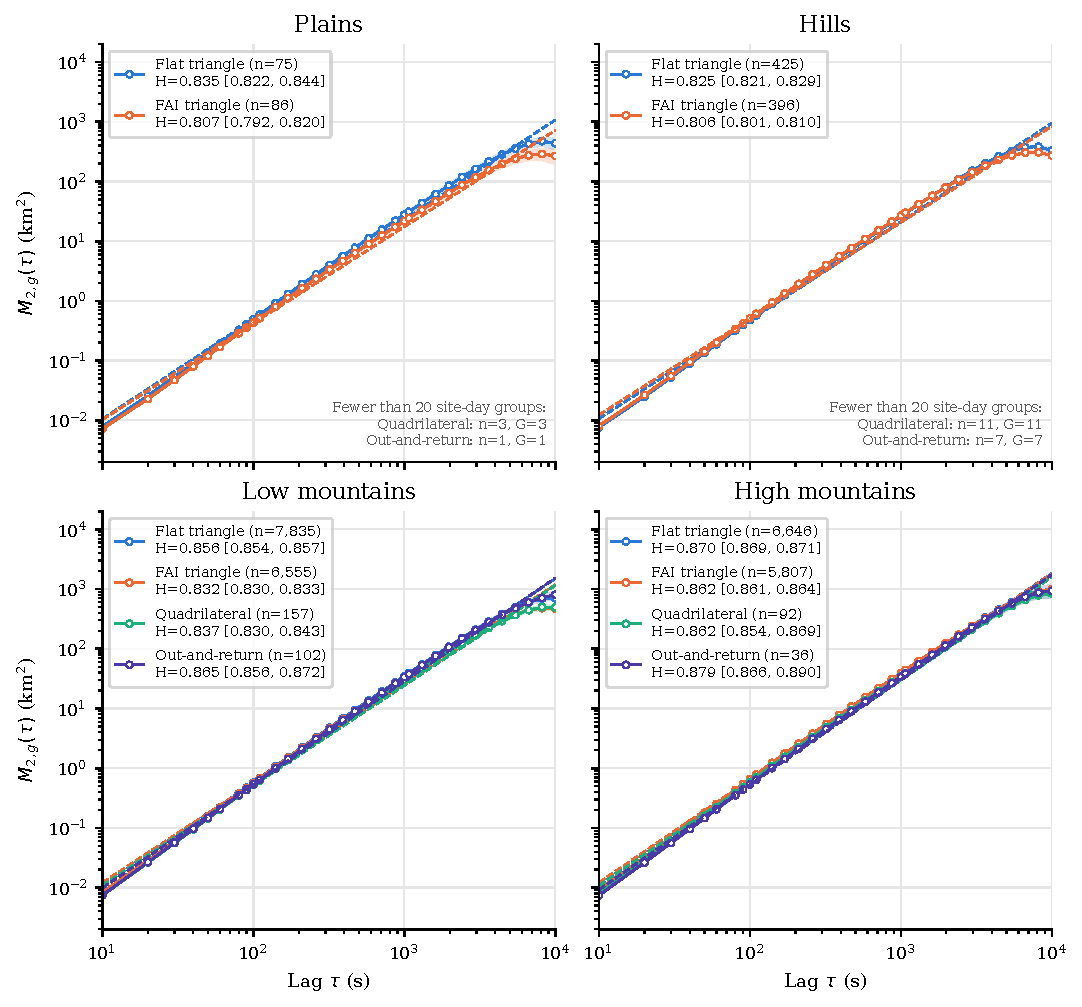
\includegraphics[width=\textwidth]{generated/ch3_route_altitude.pdf}
 \caption{Paraglider MSD $M_{2,g}(\tau)$ of Eq.~\eqref{eq:conditional-msd} by
 declared closed-route type, one panel per initial-altitude class. Solid curves
 join the equal-flight estimates, shaded bands give pointwise 90\% intervals, and
 dashed lines are fits $M_{2,g}\propto\tau^{2H_g}$ over 10--10000 s. Cells with
 fewer than \RouteMinGroups{} site--day groups are listed in their panel and not
 drawn.}
 \label{fig:route-altitude}
\end{figure}
\begin{table}[htbp]
 \centering\footnotesize\setlength{\tabcolsep}{3.5pt}
 \begin{tabular}{llrrcrr}
\toprule
Initial altitude & Route & $N$ & $G$ & $H$ [5--95\%] & $M_2(10^4)$ (km$^2$) & Year \\
\midrule
All initial altitudes & Flat triangle & 14,981 & 9,381 & 0.862 [0.861, 0.863] & 822 & 2019 \\
 & FAI triangle & 12,844 & 8,203 & 0.848 [0.847, 0.849] & 704 & 2019 \\
 & Quadrilateral & 263 & 240 & 0.847 [0.842, 0.852] & 610 & 2009 \\
 & Out-and-return & 146 & 136 & 0.868 [0.860, 0.874] & 814 & 2008 \\
\midrule
Plains & Flat triangle & 75 & 75 & 0.835 [0.822, 0.844] & 438 & 2017 \\
 & FAI triangle & 86 & 82 & 0.807 [0.792, 0.820] & 269 & 2020 \\
 & Quadrilateral & 3 & 3 & -- & -- & 2008 \\
 & Out-and-return & 1 & 1 & -- & -- & 2006 \\
\midrule
Hills & Flat triangle & 425 & 399 & 0.825 [0.821, 0.829] & 330 & 2018 \\
 & FAI triangle & 396 & 364 & 0.806 [0.801, 0.810] & 271 & 2018 \\
 & Quadrilateral & 11 & 11 & -- & -- & 2009 \\
 & Out-and-return & 7 & 7 & -- & -- & 2008 \\
\midrule
Low mountains & Flat triangle & 7,835 & 4,876 & 0.856 [0.854, 0.857] & 703 & 2019 \\
 & FAI triangle & 6,555 & 3,894 & 0.832 [0.830, 0.833] & 467 & 2019 \\
 & Quadrilateral & 157 & 143 & 0.837 [0.830, 0.843] & 493 & 2009 \\
 & Out-and-return & 102 & 92 & 0.865 [0.856, 0.872] & 804 & 2007 \\
\midrule
High mountains & Flat triangle & 6,646 & 4,160 & 0.870 [0.869, 0.871] & 998 & 2020 \\
 & FAI triangle & 5,807 & 3,950 & 0.862 [0.861, 0.864] & 1008 & 2020 \\
 & Quadrilateral & 92 & 85 & 0.862 [0.854, 0.869] & 844 & 2009 \\
 & Out-and-return & 36 & 36 & 0.879 [0.866, 0.890] & 938 & 2008 \\
\bottomrule
\end{tabular}

 \caption{Closed-route transport by initial altitude: flights $N$, site--day
 groups $G$, effective exponent $H$ with its 90\% interval, MSD at $10^4$ s and
 median launch year. The first block pools the altitude classes. Dashes mark
 cells with fewer than \RouteMinGroups{} groups.}
 \label{tab:route-altitude}
\end{table}

\paragraph{Two labels confined to the early seasons.}
In the catalogue, the quadrilateral and out-and-return labels almost vanish after
\RouteLastFourLabelYear: \RouteQuadrilateralEarlyPct\% and
\RouteOutAndReturnEarlyPct\% of these flights date from \RouteLastFourLabelYear{}
or earlier, against \RouteFlatTriangleEarlyPct\% and \RouteFaiTriangleEarlyPct\%
of the flat and FAI triangles. Comparing them with the triangles therefore also
compares older flights with recent ones, which can differ in equipment,
recorders and pilots. Table~\ref{tab:route-early} repeats the comparison with all
four routes restricted to flights up to \RouteLastFourLabelYear. Enough support
remains for the pooled altitudes and for the two mountain classes.

\begin{table}[htbp]
 \centering\footnotesize\setlength{\tabcolsep}{3.5pt}
 \begin{tabular}{llrrcrr}
\toprule
Initial altitude & Route & $N$ & $G$ & $H$ [5--95\%] & $M_2(10^4)$ (km$^2$) & Year \\
\midrule
All initial altitudes & Flat triangle & 770 & 633 & 0.855 [0.851, 0.858] & 663 & 2010 \\
 & FAI triangle & 534 & 443 & 0.835 [0.831, 0.839] & 526 & 2010 \\
 & Quadrilateral & 263 & 240 & 0.847 [0.842, 0.852] & 610 & 2009 \\
 & Out-and-return & 143 & 134 & 0.869 [0.862, 0.875] & 829 & 2007 \\
\midrule
Low mountains & Flat triangle & 454 & 371 & 0.847 [0.841, 0.852] & 558 & 2010 \\
 & FAI triangle & 316 & 261 & 0.821 [0.816, 0.825] & 353 & 2010 \\
 & Quadrilateral & 157 & 143 & 0.837 [0.830, 0.843] & 493 & 2009 \\
 & Out-and-return & 100 & 91 & 0.866 [0.857, 0.873] & 817 & 2007 \\
\midrule
High mountains & Flat triangle & 266 & 225 & 0.869 [0.864, 0.873] & 895 & 2010 \\
 & FAI triangle & 193 & 160 & 0.854 [0.846, 0.861] & 836 & 2010 \\
 & Quadrilateral & 92 & 85 & 0.862 [0.854, 0.869] & 844 & 2009 \\
 & Out-and-return & 35 & 35 & 0.881 [0.868, 0.891] & 963 & 2008 \\
\bottomrule
\end{tabular}

 \caption{As Table~\ref{tab:route-altitude}, restricted to flights up to
 \RouteLastFourLabelYear, the seasons in which all four route labels occur.
 Only altitude classes with at least two supported routes are shown.}
 \label{tab:route-early}
\end{table}

\begin{itemize}
 \item \textbf{FAI triangles have smaller $H$ than flat triangles in every
 altitude class.} The paired differences $H_{\rm FAI}-H_{\rm flat}$ are
 \RouteFaiTriangleFlatTriangleAltZeroDelta{} in Plains,
 \RouteFaiTriangleFlatTriangleAltOneDelta{} in Hills,
 \RouteFaiTriangleFlatTriangleAltTwoDelta{} in Low mountains and
 \RouteFaiTriangleFlatTriangleAltThreeDelta{} in High mountains. All four exclude
 zero, and the difference persists in the early seasons,
 \RouteFaiTriangleFlatTriangleEarlyAllDelta{} with altitudes pooled. The gap
 narrows in High mountains: the Low mountains gap minus the High mountains gap
 is \RouteFaiTriangleFlatTriangleAltTwoAltThreeDelta{}. The Plains, Hills and
 Low mountains gaps are not resolved from one another.

 \item \textbf{Within the same seasons, out-and-return flights have the largest
 $H$ and FAI triangles the smallest.} Up to \RouteLastFourLabelYear{} and with
 altitudes pooled, the order is out-and-return, flat triangle, quadrilateral,
 FAI triangle, and all six paired differences exclude zero. For example,
 out-and-return minus flat triangle is
 \RouteOutAndReturnFlatTriangleEarlyAllDelta{}, quadrilateral minus flat
 triangle \RouteQuadrilateralFlatTriangleEarlyAllDelta{} and quadrilateral
 minus FAI triangle \RouteQuadrilateralFaiTriangleEarlyAllDelta{}. The same
 order holds within Low mountains, again with all six intervals excluding zero.
 In High mountains, with \RouteOutAndReturnEarlyAltThreeN{} out-and-return and
 \RouteQuadrilateralEarlyAltThreeN{} quadrilateral flights, only three
 contrasts exclude zero: FAI minus flat triangle, and out-and-return minus
 either FAI triangle or quadrilateral.

 \item \textbf{Over all seasons, the season mix shifts these contrasts.} With
 every year included, out-and-return and flat triangles are not resolved,
 \RouteOutAndReturnFlatTriangleAllDelta{}, and quadrilaterals match FAI
 triangles, \RouteQuadrilateralFaiTriangleAllDelta{}. Triangles flown up to
 \RouteLastFourLabelYear{} have smaller exponents than the full triangle
 populations: \RouteFlatTriangleEarlyAllH{} against \RouteFlatTriangleAllH{}
 for flat triangles, \RouteFaiTriangleEarlyAllH{} against
 \RouteFaiTriangleAllH{} for FAI triangles. The all-season contrasts
 therefore combine the route difference with a change across seasons.

 \item \textbf{Both triangle types keep the closed-route altitude reversal.}
 For flat and FAI triangles alike, each lowland class has a smaller $H$ than
 each mountain class. The eight lowland-minus-mountain differences range from
 \RouteFlatTriangleAltZeroAltTwoDelta{} (flat, Plains minus Low mountains) to
 \RouteFaiTriangleAltOneAltThreeDelta{} (FAI, Hills minus High mountains), and
 all exclude zero. High mountains also exceed Low mountains, with
 Low-minus-High differences of \RouteFlatTriangleAltTwoAltThreeDelta{} for flat
 triangles, \RouteFaiTriangleAltTwoAltThreeDelta{} for FAI triangles and
 \RouteQuadrilateralAltTwoAltThreeDelta{} for quadrilaterals. The closed-route reversal of
 Section~\ref{sec:conditional-orography} therefore persists within each
 triangle type, and different proportions of flat and FAI triangles across
 altitude classes cannot explain it.
\end{itemize}

\paragraph{Interpretation.}
Within the same seasons, the ordering matches the geometric expectation at its
two ends: the route with one turnpoint has the largest $H$ and the most compact
triangle the smallest. The number of legs alone does not set the order, since
quadrilaterals lie between the two triangle types. The narrower FAI--flat gap in
High mountains is consistent with the terrain constraints discussed in
Section~\ref{sec:conditional-orography}: if slopes and ridges channel both
triangle types along similar corridors, the declared shape matters less. Both
readings remain hypotheses, because leg lengths and turn times have not been
measured. The labels are scoring categories, and the intervals retain the
limitations of Section~\ref{sec:fixed-bootstrap-reliability}.
\FloatBarrier
\subsection{Regional differences within a broad launch environment}
\label{sec:conditional-regions}
We compare Alps with Pyrenees, retaining only Low/High mountains, and
Channel Coast with Champagne-Lorraine, retaining only Plains/Hills.
This restricts the broad launch environment within each geographic comparison.
For a box $\mathcal B$ defined in Table~\ref{tab:regional-boxes} and
Figure~\ref{fig:prelim-map}a, the selections are
\begin{align}
 \mathcal C_{\mathcal B,\mathrm{mountains}}
 &=\{f\in\mathcal C_{10000}:
 (\lambda_{0f},\varphi_{0f})\in\mathcal B,\ z_{0f}\geq800\,\mathrm{m}\},\notag\\
 \mathcal C_{\mathcal B,\mathrm{lowlands}}
 &=\{f\in\mathcal C_{10000}:
 (\lambda_{0f},\varphi_{0f})\in\mathcal B,\ z_{0f}<800\,\mathrm{m}\}.
 \label{eq:regional-preselection}
\end{align}
Within the fixed cohort, this removes \CondAlpsExcluded{} flights from the Alpine
box and \CondPyreneesExcluded{} from the Pyrenean box. The lowland restriction also
removes \CondChannelCoastExcluded{} flights from Channel Coast and
\CondChampagneLorraineExcluded{} from Champagne-Lorraine. Figure legends report
the remaining counts.

\begin{figure}[htbp]
 \centering
 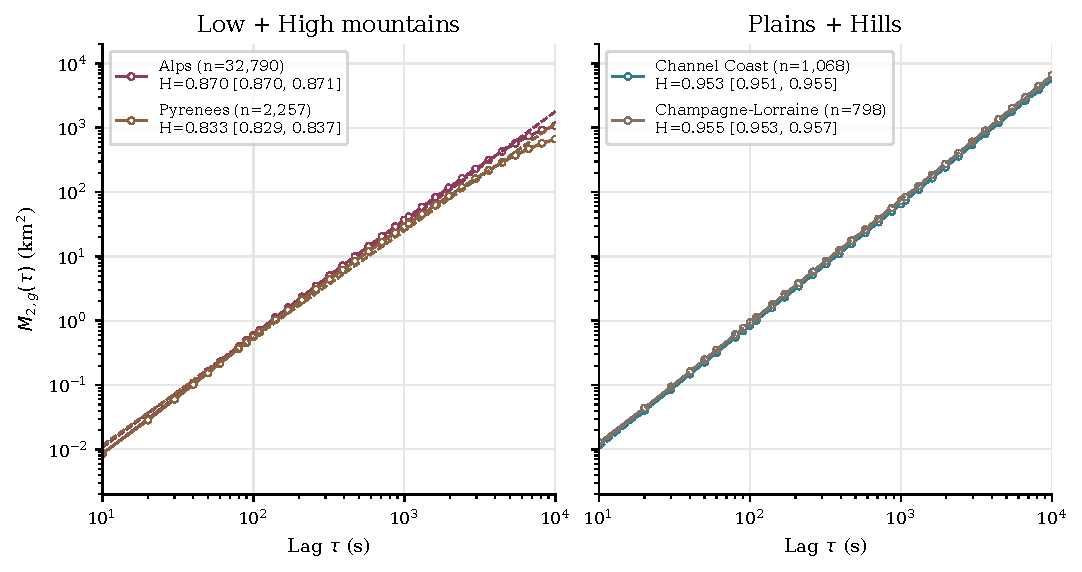
\includegraphics[width=\textwidth]{generated/ch3_conditional_regions.pdf}
 \caption{Regional paraglider MSDs. Left: Alps and Pyrenees. Right: Channel Coast
 and Champagne-Lorraine. The left panel retains only Low/High mountains within
 each box; the right retains only Plains/Hills. Circuit types and equipment
 classes are pooled. Counts and fits refer to the preselected populations;
 both panels share the same axes.}
 \label{fig:conditional-regions}
\end{figure}

The Alpine exponent is \CondAlpsH{}, against \CondPyreneesH{} in the Pyrenees.
Their paired difference is positive (Table~\ref{tab:conditional-regions}), and
Alpine flights also reach a larger MSD at long lags. Channel Coast and
Champagne-Lorraine instead give very similar exponents,
\CondChannelCoastH{} and \CondChampagneLorraineH{}. Their paired interval includes
zero, although their MSD amplitudes differ.

\begin{table}[htbp]
 \centering\small
 \begin{tabular}{@{}llc@{}}
\toprule
Setting & Contrast & $\Delta H$ [5--95\%] \\
\midrule
Mountains & Alps -- Pyrenees & $0.037\;[0.033,\,0.041]$ \\
Lowlands & Coast -- Champagne-Lorraine & $-0.002\;[-0.005,\,0.001]$ \\
\bottomrule
\end{tabular}

 \caption{Paired regional contrasts in $H$, after the terrain preselection:
 Low/High mountains for Alps--Pyrenees and Plains/Hills for the two lowland
 regions. Intervals are nominal 90\% site--day bootstrap intervals.}
 \label{tab:conditional-regions}
\end{table}

\textbf{The two lowland regions have similar growth exponents, whereas the
identity of the mountain range matters in this comparison.}

One possible explanation is a broadly distributed supply of thermal triggers
over lowlands. Sun-heated asphalt and dark, ploughed fields can heat more
rapidly than their surroundings and initiate convection~\cite{ssa_lift_sources}.
Roads, fields and other heated patches recur across different plains.
If their effective spacing and availability are statistically similar in
Channel Coast and Champagne-Lorraine, changing the region could leave the
growth exponent largely unchanged. This proposes comparable trigger
statistics across the two lowlands, rather than establishing a spatially
uniform thermal field. The source locations have not been mapped here,
and the observed similarity concerns $H$, with different MSD amplitudes.

In mountains, heated slopes and terrain-associated lift tie the places where
height can be recovered more closely to the arrangement of ridges and valleys.
Thermals can flow upslope, while wind-driven slope lift also follows the
terrain~\cite[Chapter~9]{faa_glider2024}. These distinct mechanisms both make
the geometry of the mountain range relevant to available routes.
\textbf{We interpret the lower Pyrenean $H$ and smaller long-lag MSD as
consistent with stronger constraints on net progress than in the Alps.}
Under this interpretation, the Alpine arrangement of usable slopes and
connections between them offers more freedom in choosing where to travel,
whereas the Pyrenean arrangement restricts those choices more strongly.
This is a proposed explanation of the regional contrast, not a measured
ranking of route accessibility: $H$ does not count available directions or
identify the geometry responsible for a trajectory.

Broad altitude selection still leaves different altitude distributions,
circuit proportions, equipment and weather within each regional pair.
The comparison cannot isolate terrain geometry or establish that all plains
share the same transport statistics. Testing the proposed explanation would
require independent maps of thermal triggers and usable terrain connections,
together with route comparisons under matched flight and weather conditions.

\FloatBarrier
\subsection{Beginners and experts across launch environments}
\label{sec:conditional-equipment}

We use the equipment groups defined in Section~\ref{sec:glider}:
\[
 \text{beginners}:\ \mathrm{EN\ A/B/C},\qquad
 \text{experts}:\ \mathrm{EN\ D/CCC}.
\]
Membership follows the catalogue wing class for each flight: an experienced
pilot can fly an A/B/C wing, so these labels combine an experience proxy with
equipment differences. We exclude tandem, non-certified and unclassified entries
from this comparison: \num{\CondUnknownEquipment} fixed-cohort flights enter neither
group. The retained groups contain \num{\CondBeginnersN} beginners flights and
\num{\CondExpertsN} experts flights.

\begin{figure}[htbp]
 \centering
 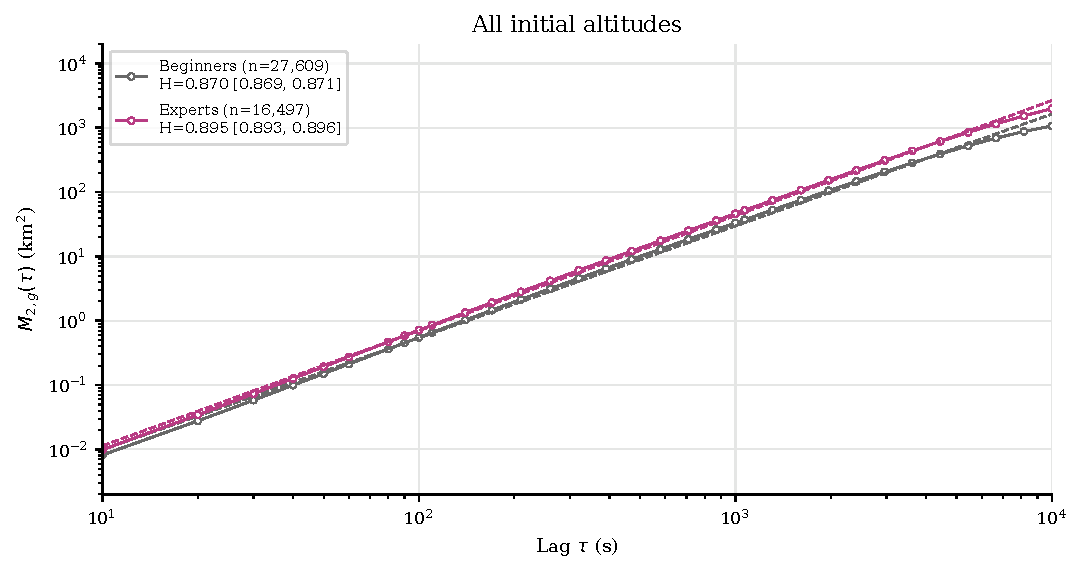
\includegraphics[width=\textwidth]{generated/ch3_conditional_equipment.pdf}
 \caption{Paraglider MSD for beginners (EN A/B/C) and experts (EN D/CCC), pooling
 regions, initial altitudes and circuit types. These names refer to equipment
 proxies; individual pilot experience is not recorded by the grouping.}
 \label{fig:conditional-equipment}
\end{figure}

Over all initial altitudes (Figure~\ref{fig:conditional-equipment}), the experts
group reaches a larger MSD and has the
larger effective exponent: \CondExpertsH{}, against \CondBeginnersH{} for
beginners. The paired difference is \CondExpertsBeginnersDelta{}.
A speed difference alone would multiply an otherwise identical MSD by a constant
and leave its log--log slope unchanged. The observed separation in $H$ therefore
also concerns the lag dependence of transport, although it cannot distinguish
pilot decisions from equipment, route or environmental differences.

Figure~\ref{fig:conditional-equipment-altitude} separates altitude classes
within the beginners group (left) and the experts group (right).

\begin{figure}[htbp]
 \centering
 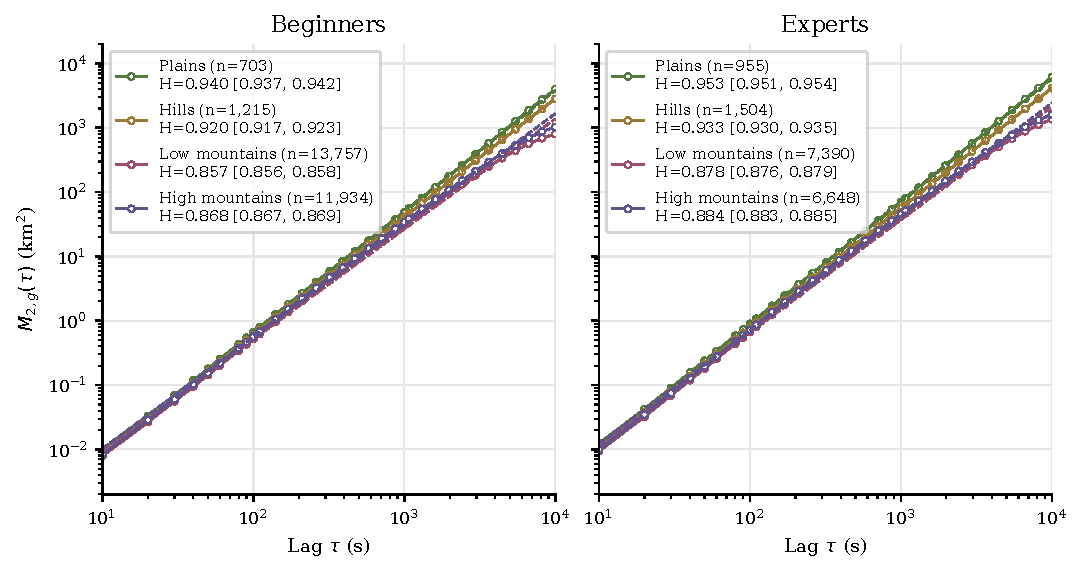
\includegraphics[width=\textwidth]{generated/ch3_conditional_equipment_altitude.pdf}
 \caption{Paraglider MSD by initial altitude for beginners (left) and experts
 (right), pooling regions and circuit types. Estimator, fit range, axes and
 uncertainty convention are the same as in Figure~\ref{fig:fixed-task}; the number
 of contributing flights is given for every curve.}
 \label{fig:conditional-equipment-altitude}
\end{figure}

For both groups the altitude ordering is that of
Figure~\ref{fig:conditional-altitude}: Plains and Hills have the larger $H$,
followed by the two mountain classes. Comparing the two panels, the experts curve
has the larger displacement amplitude at long lags and the larger $H$ in every
altitude class. All four paired differences in
Table~\ref{tab:conditional-equipment} exclude zero.

The size of the contrast depends on the environment: it is largest in Low mountains, smaller in
High mountains, and smaller again in Plains and Hills. The pooled difference is
larger than any within-class difference, showing that the all-altitude comparison
also incorporates the groups' different altitude composition and MSD amplitudes.

\begin{table}[htbp]
 \centering\small
 \begin{tabular}{@{}llc@{}}
\toprule
Setting & Contrast & $\Delta H$ [5--95\%] \\
\midrule
All altitudes & Experts -- beginners & $0.025\;[0.024,\,0.026]$ \\
Plains & Experts -- beginners & $0.013\;[0.011,\,0.015]$ \\
Hills & Experts -- beginners & $0.013\;[0.009,\,0.016]$ \\
Low mountains & Experts -- beginners & $0.021\;[0.019,\,0.022]$ \\
High mountains & Experts -- beginners & $0.016\;[0.014,\,0.017]$ \\
\bottomrule
\end{tabular}

 \caption{Experts-minus-beginners contrasts in the effective exponent, first
 pooling all altitudes and then within each class. The same bootstrap draws
 provide every contrast.}
 \label{tab:conditional-equipment}
\end{table}

To assess whether those contrasts themselves differ, define
\begin{equation}
 \Delta H_a=H_{\mathrm{experts},a}-H_{\mathrm{beginners},a},
 \qquad D_{ab}=\Delta H_a-\Delta H_b,
 \label{eq:conditional-interaction}
\end{equation}
where $a$ and $b$ denote altitude classes. We compute $D_{ab}$ within each paired
bootstrap replicate, rather than comparing the overlap of separate intervals.
The Low mountains contrast exceeds those in Plains, Hills and High mountains
with all three intervals excluding zero. The Plains--Hills difference is not
resolved, and neither is the difference between High mountains and either
lowland class at the adopted 90\% level. There is therefore evidence that the
equipment-group separation changes with launch environment, but no monotonic
increase of that separation with altitude.

These contrasts concern long flights made on different wing classes. In
particular, the beginners group does not represent the full population of
novice pilots, and circuit composition remains mixed within each altitude cell.
\FloatBarrier

\subsection{From stratified comparisons to a joint analysis}
\label{sec:conditional-synthesis}

The comparisons reveal two features that a joint analysis must account for:
\begin{itemize}
 \item \textbf{Unequal composition}: the factor proportions differ between
 groups, and each subgroup contributes according to both its abundance and
 its MSD (Eq.~\eqref{eq:fixed-msd-share}).
 \item \textbf{Interactions}: a contrast in $H$ changes with another
 factor's level, as observed for both circuit and equipment across altitude
 classes. This departure from additivity is distinct from unequal proportions.
\end{itemize}
The two-factor comparisons quantify these conditional patterns while pooling
the remaining characteristics. They cannot yet separate circuit, launch
environment and equipment jointly.

\paragraph{Factorial analysis as the next stage.}
A full \emph{factorial experiment} combines every selected level of each
factor with every level of the others~\cite{nist_full_factorial}. This permits
estimation of main effects, which summarise contrasts over specified settings
of the other factors, and interactions, which describe how those contrasts
change with the settings~\cite[Sections~9.3 and~9.7]{mohr2022statistical}.

For this archive, the corresponding \emph{factorial analysis} would cross
four altitude classes, two circuits and two equipment groups, giving 16
cells, with $H$ fitted over the same lag range in each. It would test whether
the circuit--altitude patterns persist at common equipment settings and
quantify interactions among all three factors. The observational data require
explicit weighting of unequal cells and uncertainty estimates that respect
shared flight conditions. Unmeasured weather and route selection would still
limit causal interpretation. The provisional implementation in
Section~\ref{sec:conditional-factorial}, in \emph{Experimentals}, remains under
review; none of its numerical results is used here.

\paragraph{Why this matters for group versus solo flight.}
Group flights could have a higher pooled $H$ because they contain more open
routes or different terrain and equipment mixtures. Adding group/solo status
as a fourth factor gives 32 cells and allows contrasts at common settings:
\[
 \Delta H_{a,c,e}^{\rm social}
 =H_{\mathrm{group},a,c,e}-H_{\mathrm{solo},a,c,e},
\]
where $e$ denotes equipment class. Interactions with social status would test
whether this contrast changes with circuit, altitude or equipment. Such joint
comparisons are needed to distinguish the group/solo association from these
composition effects; they require reliable social-flight labels and sufficient
support in each compared cell.
\FloatBarrier

\section{Anisotropy and principal directions}
\label{sec:fixed-anisotropy}
\emph{Reserved for the analysis of anisotropy and principal directions. The existing
PCA results remain in the experiments volume; they are not updated in this chapter.}
